\documentclass{article}
\usepackage{graphicx} % Required for inserting images
% 基础包
\usepackage[utf8]{inputenc}
\usepackage[T1]{fontenc}
\usepackage{lmodern}
\usepackage{geometry}
\setlength{\parindent}{0pt} % 全局取消缩进
\geometry{a4paper, margin=1in}

% 数学相关包
\usepackage{amsmath}
\usepackage{amssymb}
\usepackage{amsthm}
\usepackage{bm}
\usepackage{biblatex}
\addbibresource{reference.bib}

% 表格和图表
\usepackage{booktabs}   % 专业表格
\usepackage{caption}    % 图表标题
\usepackage{subcaption} % 子图
\usepackage{graphicx}   % 图片插入
\graphicspath{{figures/}} % 图片路径

\include{preamble}
\usepackage{morefloats}

% 代码显示
\usepackage{listings}
\usepackage{xcolor}
\usepackage{outlines}


% Matlab代码样式设置
\definecolor{matlabgreen}{RGB}{28,172,0}
\definecolor{matlabpurple}{RGB}{170,55,241}
\lstset{
    language=Matlab,
    basicstyle=\ttfamily\footnotesize,
    breaklines=true,
    frame=single,
    showstringspaces=false,
    numbers=left,
    numberstyle=\tiny,
    keywordstyle=\color{blue},
    commentstyle=\color{matlabgreen},
    stringstyle=\color{matlabpurple},
    rulecolor=\color{black!30},
    tabsize=4,
    captionpos=b,
    belowcaptionskip=8pt
}

% 定理环境
\newtheorem{theorem}{Theorem}[section]
\newtheorem{lemma}[theorem]{Lemma}
\newtheorem{definition}[theorem]{Definition}

%\title{Complex Systems}
%\author{Juji Li}
%\date{May 2026}


\begin{document}

\include{cover}

\tableofcontents % 自动生成目录

\clearpage

\section{Introduction}
Many-body systems driven far from equilibrium can exhibit emergent behaviour that is not evident from the local rules governing their constituent parts. In particular, certain slowly driven, dissipative systems produce intermittent responses spanning a broad range of magnitudes, from small local rearrangements to large-scale system-wide events. Understanding how such behaviour arises is a central problem in complex systems physics. In this report, this problem is examined through the Bak–Tang–Wiesenfeld (BTW) sandpile model, which provides a minimal theoretical framework for the study of self-organized criticality (SOC). SOC refers to the tendency of some extended systems to evolve dynamically towards a critical state without the need for external fine-tuning of control parameters.

\hspace{5mm}

A defining characteristic of critical states is scale invariance: the system exhibits no single preferred length or event scale, and similar statistical structure is observed across multiple orders of magnitude. One important consequence of scale invariance is the emergence of power-law behaviour in the distribution of event sizes. In such distributions, small events occur frequently, while large events remain rare but non-negligible, reflecting the absence of a characteristic scale. Power laws of this type are observed in a wide range of natural phenomena, including earthquakes, solar flares, forest fires, epidemics, and fluctuations in financial markets. Their appearance across otherwise very different systems suggests that common statistical principles may underlie diverse forms of complex collective behaviour.

\hspace{5mm}

The BTW sandpile model is therefore of particular interest because it captures these features within a mathematically simple and computationally tractable setting. Despite its highly idealised construction, the model generates avalanche dynamics whose statistical properties provide a natural setting in which to investigate SOC, non-equilibrium behaviour, and scale-free distributions. The purpose of this report is to analyse the extent to which the BTW model reproduces these characteristics, and to use it as a framework for understanding why power laws arise so naturally in slowly driven critical systems.

\subsection{Self-organized Criticality and Scale Invariance}
In 1987, Bak, Tang and Wiesenfeld introduced the concept of self-organized criticality (soc). Self-Organized Criticality refers to the phenomenon in which certain complex systems, when slowly driven, spontaneously evolve into a "critical state" without the need for precise, manual parameter tuning. And, scale invariance refers to a system appearing to possess similar structures or statistical regularities across different scales of observation, lacking any single, fixed "typical scale." The example of the Scale invariance is the Mandelbrot set. And, there are also examples from the real world, such as earthquakes and forest fires. The distribution of the magnitudes of these events often follows a power law. And \textit{if a system "looks roughly the same" at both large and small scales, then it does not favor any particular scale; and the power law is precisely the quintessential mathematical form of this "absence of a characteristic scale."} 

\subsection{Non-equilibrium Statistics}
Non-equilibrium statistical means that the system has many degrees of freedom, too many internal variables, and too complex interactions. Therefore, complex system:

\begin{itemize}
    \item  are difficult to calculate using analytical methods.
    \item to accurately calculate the complete evolution of the entire system over time.
\end{itemize}

In other words, for complex systems, we cannot calculate every single detail precisely. Therefore, we need to rely on non-equilibrium statistics methods to calculate complex systems.

\subsection{Aim}
The purpose of our research is:
\begin{itemize}
    \item establish a basic sandpile model.
    \item study self-organized criticality within the sandpile model.
    \item investigate related non-Gaussian statistics.
\end{itemize}


\clearpage

\section{Bak Tang Wiesenfeld Model}
As previously noted, modeling complex systems is exceedingly difficult; therefore, we will employ the Bak–Tang–Wiesenfeld model. Since the Bak–Tang–Wiesenfeld model (BTW model) utilizes a remarkably simple rule to simulate how complex systems spontaneously generate "avalanche-like" chain reactions, we will use it to construct our sandpile model.

Now we building the BTW model describes sand pile. The system consists of an $N \times M$ grid of points:

\begin{itemize}
    \item At each point $(i, j)$, there is a grains of sand, where $i \in [1,..,N]$, $j\in[1,...,M]$, and $t\in \mathbf{N}^0$.
    \item At each time step t, a new gain of sand is added to random site in the lattice causing the sand piles at each site to grow.
    \item $p_t(i,j)$ indicates the number of sand grains at this position at time $t$.
    \item The entire system is driven slowly—not by adding a large amount all at once, but by adding it grain by grain.
    \item If the height of a single sand pile reaches 4 or higher, the pile will topple, distributing four grains of sand to the four adjacent positions:

    \begin{align}
    p_t(i,j) =p_t(i,j)-4 \\
    p_t (i\pm1,j) = p_t(i\pm1, j)+1 \\
    p_t (i,j\pm1) = p_t(i, j\pm1)+1
    \end{align}

    \item If the pouring point is located at the edge, any sand that spills off the table is removed by the system.

    \item If an adjacent cell already contains four grains of sand, that adjacent cell will also spill over.
\end{itemize}

BTW satisfies the following conditions of self-organized criticality:

\begin{itemize}
    \item Slow driven: sand is added only once per second.
    \item Local threshold: Stability is lost once the height reaches 4.
    \item Local interaction: Only affects the upper, lower, left, and right neighbors.
    \item Chain reaction: Small perturbations can trigger large-scale avalanches.
    \item Boundary dissipation: Excess sand can leave the system.
    \item No fine-tuning required: Once the rules are fixed, the system will evolve to the vicinity on its own.
\end{itemize}

We must stipulate that the boundaries of the table are finite for the sandpile model to be meaningful. Because if the boundaries of the sandpile model are infinite, then:

\begin{itemize}
    \item The sand will remain on the table forever.
    \item The sand on the table will keep increasing, and the system can never reach a stable equilibrium.
\end{itemize}

If the grid is infinite, but we add sand only within a finite region, this sandpile model will:

\begin{itemize}
    \item Sand will spread from within its boundaries into the infinite; as time passes, the table will recede into infinity.
    \item The disturbed region will grow larger and larger, until it reaches infinity.
    \item If we consider only the situation within a finite region, then a steady state exists within that region. However, if we consider an infinite lattice, then no steady state exists for the system.
\end{itemize}

In other words, finite boundaries allow sand to "leak out," thereby giving rise to a steady state. If no sand were to "leak out," the system is hard to be a steady state, as the quantity of sand would continue to increase indefinitely.

\clearpage

\subsection{Average height}
Without simulation, the steady-state system would be:

\begin{itemize}
    \item The average height will start from 0 and increase.
    \item After continuously increasing, the average height will oscillate within a small range, indicating that the system has entered a steady state.
\end{itemize}

Calculations show that the steady-state average height will be 2.175 (The calculation shown in appendix).


We define the average height of each pile to be:

\begin{equation}
    <p_t> := \frac{1}{NM} \sum_{i,j} p_t(i,j).
\end{equation}

And we using Matlab to plot the graph, and the estimated steady-state is $<p_t> = 2.1126$, which is close to 2.175:
\begin{figure}[htpt]
    \centering
    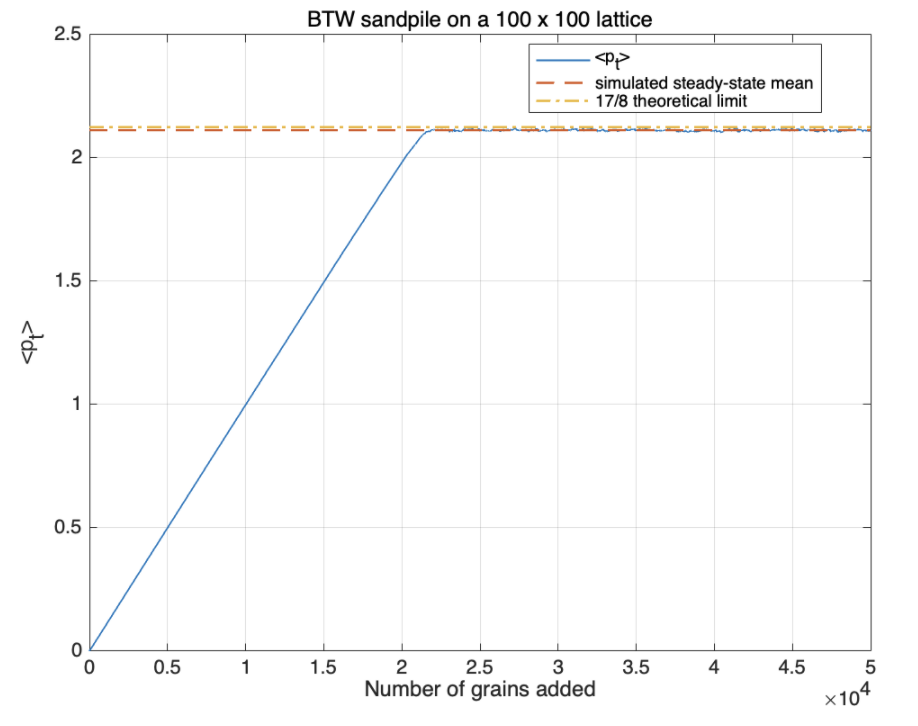
\includegraphics[width=0.4\linewidth]{image.png}
    \caption{Simulation of sand pile model}
    \label{fig:placeholder}
\end{figure}

\clearpage

\subsection{Steady State and Statistically Stationary State, and an Equilibrium State}

A \textbf{steady state} typically refers to a condition in which certain macroscopic quantities of a system no longer change systematically over time. Such as the average height:

\begin{align}
    <p_t> := \frac{1}{NM} \sum_{i,j} p_t(i,j).
\end{align}

This means the height will rise, but eventually, it will fluctuate around a certain value. At this point, it can be said to have entered a kind of steady state. Note that, the specific microscopic configuration of the sand pile remains in constant flux; every addition or pouring of sand alters the height of the lattice points. Consequently, it does not represent a "completely static" steady state, but rather a state in which the macroscopic statistical quantities remain stable. And the Steady-State Altitude Distribution is Figure 2. By simulation, height probabilities after burn-in is: $P(0) = 0.0768$, $P(1) = 0.1808$, $P(2) = 0.3096$ and $P(3) = 0.4327$.


\begin{figure}[htbp]
\centering
    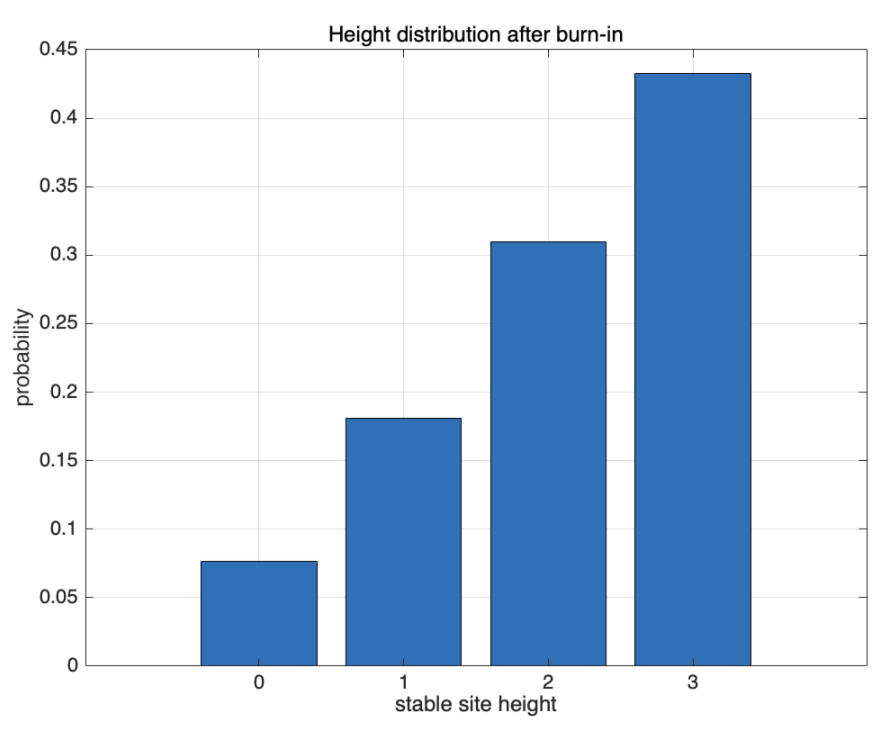
\includegraphics[width=0.4\linewidth]{image2.png}
    \caption{the Steady-State Altitude Distribution}
    \label{fig:placeholder}
\end{figure}

A \textbf{statistically stationary state} refers to a specific state of a system in which the system's actual configuration continues to evolve, yet its statistical properties remain invariant over time. A statistically stationary state is better suited than a conventional "steady state" for describing the BTW model. For instance, once the system enters a statistically stationary state: 

\begin{itemize}
    \item $<p_t>$ fluctuates around a specific value.
    \item The height distribution $P(p=0)$, $P(p=1)$, $P(p=2)$ and $P(p=3)$ remains essentially stable.
    \item The distributions of avalanche size, area, damage, and length are also essentially stable.
    \item It is not that every step is identical, but rather that long-term statistical patterns remain stable.
\end{itemize}

The concept of an \textbf{equilibrium state} is a stronger one. In a true equilibrium state, the system is subject to neither continuous external driving forces nor continuous dissipation or net flows. For instance, in thermodynamic equilibrium, the system exhibits no continuous flow of energy or matter, and typically satisfies the condition of detailed balance.

BTW model is not in a steady state, because:
\begin{itemize}
    \item The external environment continuously adds sand to the system;
    \item The boundaries are constantly liable to leak sand;
    \item Avalanches occur incessantly within the system;
    \item There is a continuous process of input and dissipation.
\end{itemize}
Therefore, the state attained by the BTW model is not an equilibrium state, but rather a non-equilibrium statistically stationary state.

\hspace{2mm}

Incidentally, the BTW model does not reach a true equilibrium state. Instead, after undergoing a transient period that is, a transitional phase it attains a statistically stationary state.

In this state:
\begin{itemize}
    \item The average height no longer continues to rise;
    \item The single grain of sand added at each step is, on average over the long term, dissipated at the boundaries;
    \item The statistical distribution of avalanches becomes stable;
    \item The system exhibits SOC that is, Self-Organized Criticality.
\end{itemize}

\subsection{Avalanche observables}
\textbf{Topples} refers to the total number of toppling events that occur during a single avalanche. If the same grid point topples twice, it is counted twice.

\hspace{2mm}

\textbf{Area} refers to the number of distinct grid points that experienced a toppling event during the avalanche. It counts unique sites; if the same grid point topples three times, its contribution to the Area remains just 1.

\hspace{2mm}

\textbf{Loss} refers to the number of sand grains that fall out of the system across its boundaries during a specific avalanche event. For instance, when a grid point located at the boundary \textit{topples}, it typically attempts to distribute one grain to each of its four neighbors; however, if a specific direction lacks a neighboring cell, that particular grain is lost.

\begin{itemize}
    \item Toppling at an edge grid point: Typically results in a loss of 1 grain;
    \item Toppling at a corner grid point: Typically results in a loss of 2 grains;
    \item Toppling at an internal grid point: Results in a loss of 0 grains.
\end{itemize}

\hspace{2mm}

\textbf{Length} is a quantity used to characterize the spatial scale of an avalanche. Centered on the lattice site where the initial topple occurred, it is defined as the maximum distance from that site to any of the toppled sites. If the Manhattan distance—specifically, the $L_1$ norm is employed:

\begin{align}
    l := \max_{(i,j) \in A}(|i-i_0|+|j-j_0|),
\end{align}
where $(i_0, j_0)$ is the starting point of the avalanche, and $A$ is the set of all grid points where toppling has occurred. \\

This definition is quite natural; since, in the BTW model, sand grains propagate only vertically and horizontally rather than diagonally the Manhattan distance aligns more closely with the lattice propagation rules than the Euclidean distance does. \\

If using Euclidean distance, it can also be defined as:

\begin{align}
    l = \max_{(i,j) \in A} \sqrt{(i-i_0)^2+(j-j_0)^2}.
\end{align}

We chose Euclidean distance to define the length of an avalanche because we wanted to characterize its actual geometric extent in space, rather than the number of steps the sand grains took as they propagated across the lattice. Because:

\begin{itemize}
    \item It is more akin to "length" in real space.
    \item It characterizes the spatial scale of an avalanche, rather than its propagation path.
    \item It avoids overestimating distances in diagonal directions. For example, the Manhattan distance from $(0,0)$ to $(1,1)$ is:
    \begin{align}
        \sqrt{1^2+1^2} = \sqrt{2}
    \end{align}
\end{itemize}

\subsection{Time sampling and Ensemble sampling}
\textbf{Time sampling} involves observing the same system over an extended period. For example, one might simulate a $50 \times 50$ sand pile, run it for $100,000$ steps, and then record the avalanche size at each step. Mathematically: 

\begin{align}
    \bar{O}_{time} = \frac{1}{T} \sum^T_{t=1} O_t.
\end{align}

\textbf{Ensemble sampling} involves simultaneously considering a multitude of independent systems. For example, you might run $1,000$ separate $50 \times 50$ sand pile simulations using different random seeds; once each system has reached a steady state, you then record their respective avalanche sizes. Mathematically:

\begin{align}
    <O>_{ensemble} = \sum_x O(x) P(x).
\end{align}

If a system is ergodic, then observing a single system over a long period should yield the same statistical results as observing a large number of independent systems:

\begin{align}
    \bar{O}_{time} = <O>_{ensemble}
\end{align}

When time sampling and ensemble sampling are equivalent, we require:
\begin{itemize}
    \item The system has passed its initial transient phase;
    \item The simulation duration is sufficiently long;
    \item The random sampling of initial states enables the system to explore all relevant recurrent states;
    \item The system has not become trapped within a specific region of the state space.
\end{itemize}
For a finite-sized, open-boundary BTW model with random sand addition, it can generally be regarded as ergodic on its recurrent configurations. Consequently, in practical simulations, an ensemble average can typically be approximated using a sufficiently long time series.

\clearpage

\subsection{Frequency of Avalanche}
In the BTW model, the size of an avalanche lacks a fixed characteristic scale; consequently, we expect these distributions not to be Gaussian, but rather heavy tailed typically approximated by a power law with a finite-size cutoff. The general form is:

\hspace{2mm}

\textbf{Topples distribution}: Let $s=$number of topples indicates the total number of topples that occurred during a single avalanche. We then have the expected distribution is:
\begin{align}
    P(s) \sim s^{-\tau_s} 
\end{align}
in a finite system, we have:
\begin{align}
    P(s) \sim s^{-\tau_s}f_s(\frac{s}{s_c})
\end{align}
It is a cutoff resulting from the finite system size. In other words, small avalanches are numerous, while large avalanches are rare; however, large avalanches are still more common than predicted by a Gaussian distribution. By simulation: 
\begin{figure}[htbp]
    \centering
    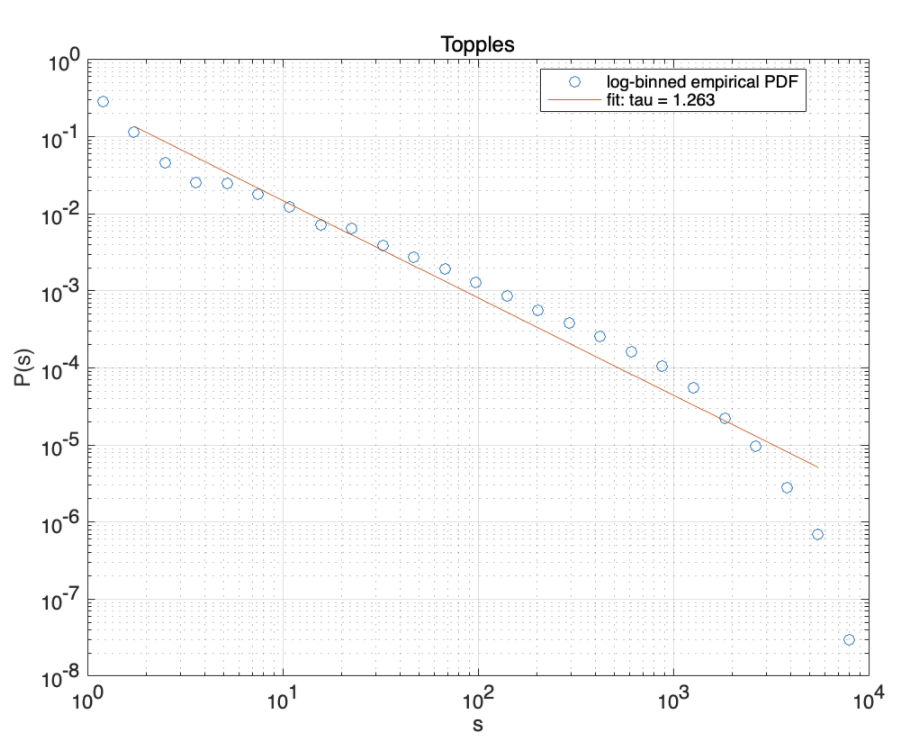
\includegraphics[width=0.32\linewidth]{image3.png}
    \caption{log-binned distribution and power-law fit of topples}
    \label{fig:placeholder}
\end{figure}

\textbf{Area distribution}: let $a=$ number of unique toppled sites indicates the number of distinct grid points at which a topple occurred during a single avalanche. Expectation:

\begin{align}
    P(a) \sim a^{-\tau_a}
\end{align}

Note that "topples" and "area" are not exactly the same. If the same point topples multiple times, it contributes multiple times to the topples count, but only once to the area. We then have:

\begin{align}
    s \geq a
\end{align}
And By simulation, we have:
\begin{figure}[htbp]
    \centering
    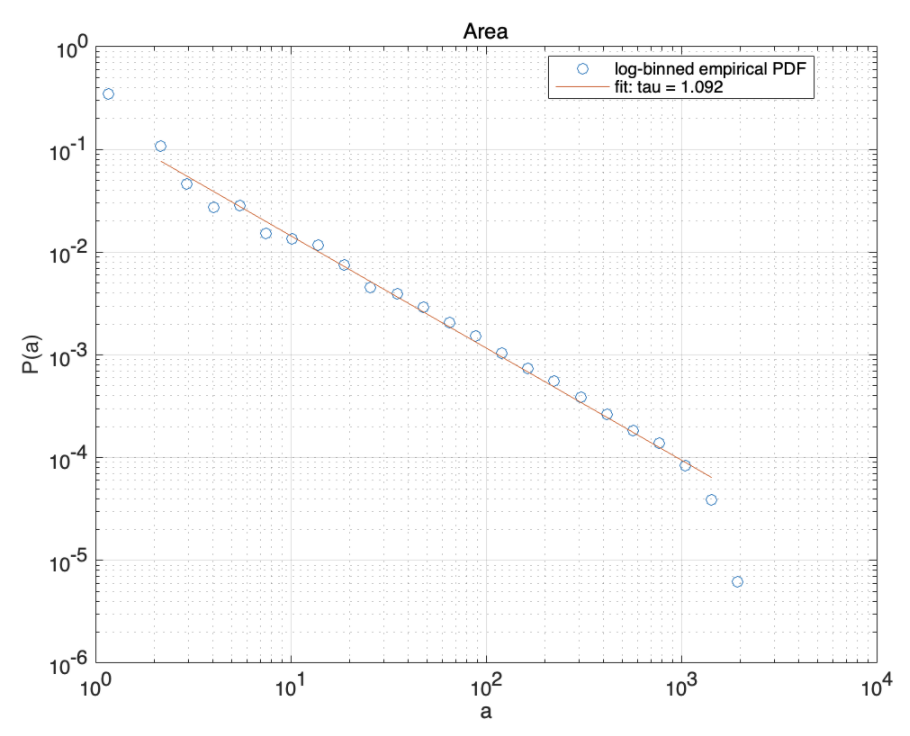
\includegraphics[width=0.32\linewidth]{image4.png}
    \caption{log-binned distribution and power-law fit of area}
    \label{fig:placeholder}
\end{figure}

\clearpage

\textbf{Loss distribution}: let $d=$ number of grains lost at the boundary. Loss occurs only when an avalanche reaches the boundary. Consequently, the distribution of loss is not exactly identical to that of topples, area, or length. Many avalanches may occur entirely within the interior; So:

\begin{align}
    d = 0
\end{align}
For positive losses specifically the region where $d > 0$ one typically observes a broad distribution or behavior approximating a power law; however, this region is more strongly influenced by boundary effects. By simulation we have:

\begin{figure}[htbp]
    \centering
    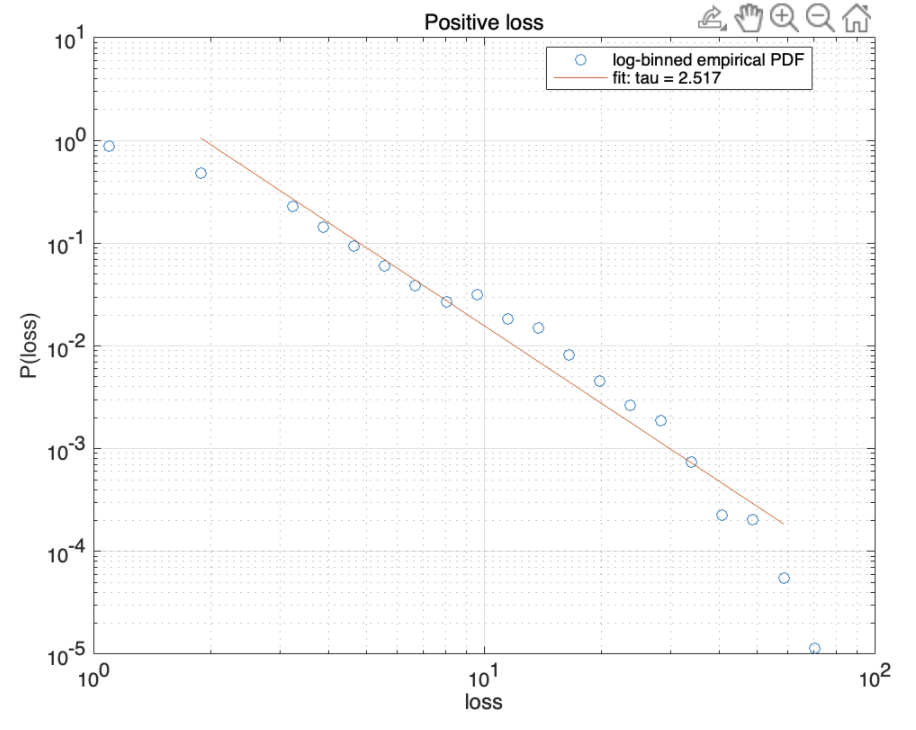
\includegraphics[width=0.32\linewidth]{image5.png}
    \caption{log-binned distribution and power-law fit of positive loss}
    \label{fig:placeholder}
\end{figure}

\textbf{Length distribution}: Here, we choose to define the avalanche length using the Euclidean distance. If an avalanche begins at point $(i_0,j_0)$, and the set of all grid points where toppling has occurred is denoted as $A$, then we define it as follows:

\begin{align}
    l = \max_{(i,j)\in A}\sqrt{(i-i_0)^2+(j-j_0)^2}
\end{align}
This definition measures the geometric extent of the avalanche in two-dimensional space, rather than the number of steps taken along the lattice. The expected length distribution is:

\begin{align}
    P(l) \sim l^{-\tau l}
\end{align}
There will also be a finite-size cutoff. By simulation we have:
\begin{figure}[htbp]
    \centering
    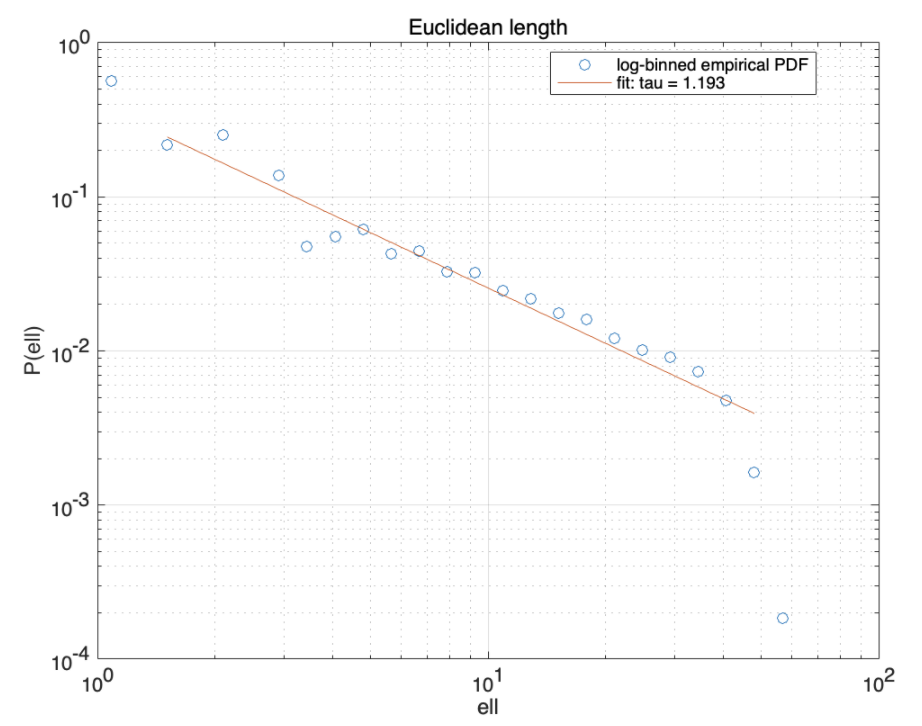
\includegraphics[width=0.32\linewidth]{image6.png}
    \caption{log-binned distribution and power-law fit of Euclidean length;}
    \label{fig:placeholder}
\end{figure}





\textbf{Power Law}: 
If a variable $x$ satisfies:
\begin{align}
    P(x) \sim x^{-\tau}
\end{align}
Then, taking the logarithm of both sides:
\begin{align}
    log P(x) = - \tau log x+C
\end{align}
Therefore, on a log-log plot, if the intermediate region is approximately a straight line, the slope is $-\tau$. So, $\tau = -slope$. In the MATLAB simulation, a log-binned power-law fit has been applied to the topples, area, length, and positive loss, yielding the approximate exponents.

\subsection{Correlations of avalanche observables}
\textbf{Topples} and \textbf{area} should exhibit a strong positive correlation. This is because the greater the number of grid points involved in a single avalanche, the higher the total number of topples tends to be. However, the two are not exactly identical:

\begin{align}
    topples \geq area
\end{align}
Because the same grid point can topple multiple times.\\

\textbf{Area} and \textbf{length} should also be positively correlated. If an avalanche propagates further, it will typically cover a larger number of grid points. This relationship can be expressed using a scaling relation:

\begin{align}
    a \sim l^D,
\end{align}

Here, $D$ represents the effective dimension or fractal dimension of the avalanche cluster. If the avalanche region is relatively compact, it may approach:

\begin{align}
    a \sim l^2,
\end{align}
If the avalanche cluster is fractal-shaped, then $D < 2$.

\hspace{2mm}

\textbf{Topples} and \textbf{length} should also be positively correlated. An avalanche that propagates over a greater distance typically requires a larger number of topples. However, if certain regions undergo repeated toppling, the actual number of topples may exceed the value predicted solely based on length.\\

Loss also exhibits a positive correlation trend with topples, area, and length; however, this correlation is weaker and more susceptible to boundary effects. The reason is:

\begin{itemize}
    \item If an avalanche does not reach the boundary, the loss is zero.
    
    \item Even if an avalanche is substantial in size, it may result in no loss if it remains confined within the system.
    
    \item If an avalanche originates near the boundary, a loss may occur even if the avalanche itself is not large in scale.
\end{itemize}
\begin{figure}[htbp]
    \centering
    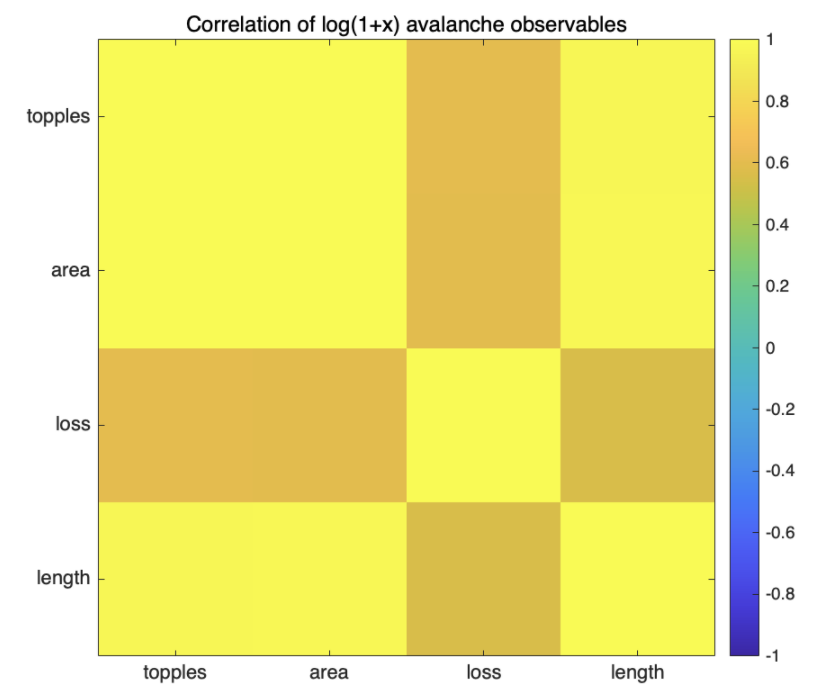
\includegraphics[width=0.5\linewidth]{image7.png}
    \caption{The correlation matrix of four avalanche observables}
    \label{fig:placeholder}
\end{figure}

\clearpage

\subsection{Abelian Property}
The BTW model has an important mathematical property: the toppling operations are Abelian. This means that the final stable configuration does not depend on the order in which unstable sites are toppled, provided that only legal topplings are performed.\\

For example, after toppling the central site in the configuration shown in the notes, the system contains two unstable sites at the top-middle and bottom-middle positions. If the top site is toppled first and then the bottom site, the final stable configuration is the same as if the bottom site is toppled first and then the top site. Thus the order of toppling does not affect the relaxed configuration.\\

This can be written using the toppling matrix. Let \(p:L\to\mathbb{N}^0\) be the sandpile configuration and let \(T_x\) denote a toppling at site \(x\). If \(\Delta(x,y)\) is the toppling matrix, then

\[
(T_xp)(y)=p(y)-\Delta(x,y).
\]

For two topplings at sites \(x\) and \(z\),

\[
(T_zT_xp)(y)=p(y)-\Delta(x,y)-\Delta(z,y),
\]

whereas

\[
(T_xT_zp)(y)=p(y)-\Delta(z,y)-\Delta(x,y).
\]

Since addition is commutative, these two expressions are equal. Therefore the toppling operations commute. This Abelian property greatly simplifies numerical simulations, because any legal order of relaxing unstable sites gives the same final stable state. By simulation we have the two orders give the same final configuration, and the simulation code shown in Appendix. \\

Initial condition $p_0$:
\[
\begin{matrix} 
2 & 3 & 1 \\
1 & 4 & 0 \\
2 & 3 & 2
\end{matrix}
\]

After toppling the centre site:

\[
\begin{matrix} 
2 & 4 & 1 \\
2 & 0 & 1\\
2 & 4 & 2
\end{matrix}
\]


upper site then lower site and lower site then upper site is the same:
\[
\begin{matrix} 
3 & 0 &2 \\
2 & 2 & 1\\
3 & 0 & 3
\end{matrix}
\]

The simulation confirms the Abelian property of the BTW sand pile model. Relaxing the same unstable configuration using different legal toppling orders gives the same final stable configuration. In addition, the toppling-count matrix and the total boundary loss are also unchanged. This confirms that the avalanche observables used in the simulation are independent of the arbitrary choice of toppling order.

\clearpage

\subsubsection{toppling matrix and condition of toppling matrix}
The Condition of toppling matrix is:

\begin{align}
    \forall x,y\in L \quad \mbox{where} \quad x \neq y , \quad \Delta (y,x) >0, \\
    \forall x \in y, \quad \Delta (x,x) < 0,\\
    \forall x \in L, \sum_{y\in L} \Delta (x,y) \leq 0, \\
    \sum_{x,y \in L} \Delta (x,y) < 0.
\end{align}

The toppling matrix is written with the sign convention that toppling site \(x\) changes the height at site \(y\) by \(\Delta(x,y)\). Thus a negative diagonal entry means that the toppled site loses sand, while positive off-diagonal entries mean that neighbouring sites gain sand.\\

Condition (24),
\[
\Delta(x,y)=\Delta(y,x)\ge 0,\quad x\ne y,
\]
means that a toppling at one site can only add grains to other sites, not remove grains from them. The symmetry means that the coupling between two neighbouring sites is reciprocal, as expected for an undirected lattice. This is necessary for the standard BTW model because sand is redistributed locally and isotropically to neighbouring sites.\\

Condition (25),
\[
\Delta(x,x)<0,
\]
means that when site \(x\) topples, it loses grains. This is necessary because a toppling must reduce the height of the unstable site; otherwise toppling would not resolve the instability. \\

Condition (26),
\[
\sum_{y\in L}\Delta(x,y)\le 0,
\]
means that a single toppling cannot create sand. If the row sum is zero, the toppling is conservative within the lattice. If the row sum is negative, sand is dissipated, usually because the site is on the boundary and some grains are sent outside the system. This is necessary for a physical sandpile model with boundary dissipation. \\

Condition (27),
\[
\sum_{x,y\in L}\Delta(x,y)<0,
\]
means that the finite system has net dissipation somewhere. This is necessary for a driven finite sandpile to reach a statistically stationary state. Without dissipation, adding grains repeatedly would make the total mass grow without bound, and stabilization after continuous driving would not be possible.

\subsubsection{Toppling matrix in the btw model}

For the BTW model on a \(d\)-dimensional cubic lattice, each site has \(2d\) nearest-neighbour directions. The toppling matrix is
\[
\Delta(x,y)=
\begin{cases}
-2d, & x=y,\\
1, & x,y\text{ are nearest neighbours},\\
0, & \text{otherwise}.
\end{cases}
\]

This definition exactly represents the BTW toppling rule. When site \(x\) topples, it loses \(2d\) grains and each in-lattice nearest neighbour receives one grain. If a nearest-neighbour direction points outside the finite lattice, that grain is lost from the system.

The matrix satisfies the conditions in Eq. (24-27):

\begin{itemize}
    \item For \(x\ne y\), \(\Delta(x,y)\) is either 0 or 1, so it is non-negative. Nearest-neighbour adjacency is symmetric, so \(\Delta(x,y)=\Delta(y,x)\).
    \item The diagonal entry is \(\Delta(x,x)=-2d<0\).
    \item For any site \(x\),
  \[
  \sum_{y\in L}\Delta(x,y)=-2d+n_x\le 0,
  \]
  where \(n_x\le 2d\) is the number of nearest neighbours of \(x\) that are still inside \(L\). Interior sites have row sum 0; boundary sites have negative row sum.
  \item Since the lattice is finite with open boundaries, at least one site has \(n_x<2d\). Therefore
  \[
  \sum_{x,y\in L}\Delta(x,y)<0.
  \]

The stability threshold is
\[
k=-\Delta(x,x)=2d.
\]
For the two-dimensional square lattice used in the simulations, \(d=2\), so
\[
k=4.
\]
\end{itemize}

Thus a site is stable if \(p(x)<4\) and unstable if \(p(x)\ge 4\).

\subsubsection{$T_x$ and $T_{x'}$ commute for unstable configurations}
Let \(T_x\) denote a legal toppling at site \(x\). With the sign convention in the notes,
\[
(T_xp)(y)=p(y)+\Delta(x,y),
\]
provided that \(p(x)\ge -\Delta(x,x)=k\).\\

Suppose two distinct sites \(x\) and \(x'\) are both unstable in configuration \(p\). Since off-diagonal entries of \(\Delta\) are non-negative, toppling one of these sites cannot decrease the height of the other. Therefore both orders of toppling are legal.\\

Now compute the two possible orders. First topple \(x\), then \(x'\):
\[
(T_{x'}T_xp)(y)
=p(y)+\Delta(x,y)+\Delta(x',y).
\]
First topple \(x'\), then \(x\):
\[
(T_xT_{x'}p)(y)
=p(y)+\Delta(x',y)+\Delta(x,y).
\]
These expressions are equal because addition is commutative. Hence
\[
T_{x'}T_xp=T_xT_{x'}p.
\]
Therefore legal toppling operations commute.

\hspace{2mm}

\subsubsection{Well defined}

The stabilization operator \(\mathcal{T}\) maps an unstable configuration to the stable configuration obtained after all legal topplings have been performed. To show that \(\mathcal{T}\) is well defined, we must show that the final stable configuration is independent of the legal toppling order.\\

For any legal stabilizing sequence, define the odometer function \(u(x)\) to be the number of times site \(x\) is toppled. If a sequence with odometer \(u\) stabilizes \(p\), the final configuration is
\[
q(y)=p(y)+\sum_{x\in L}u(x)\Delta(x,y).
\]

Let \(a(x)\) be the odometer of one legal stabilizing sequence \(\alpha\). We first show that no other legal sequence \(\beta\) can topple any site more often than \(\alpha\). Suppose, for contradiction, that \(\beta\) is the first legal sequence to exceed \(a(x)\) at some site \(x\). Immediately before this extra toppling at \(x\), the number of previous topplings at \(x\) is exactly \(a(x)\), while every other site \(z\) has been toppled no more than \(a(z)\) times. The height at \(x\) at this moment is therefore no greater than its height in the stable configuration produced by \(\alpha\), because off-diagonal entries \(\Delta(z,x)\) are non-negative. But the configuration produced by \(\alpha\) is stable, so the height at \(x\) is below threshold. This contradicts the assumption that the extra toppling at \(x\) was legal. Therefore any legal sequence has odometer \(\le a\) componentwise. If there are two legal stabilizing sequences with odometers \(a\) and \(b\), applying the same argument in both directions gives
\[
b\le a
\quad\text{and}\quad
 a\le b.
\]
Hence
\[
a=b.
\]
Thus every legal stabilizing sequence topples each site the same number of times. Consequently the final stable configuration
\[
p'(y)=p(y)+\sum_{x\in L}a(x)\Delta(x,y)
\]
is unique.\\

Therefore the stabilization operator \(\mathcal{T}\) is well defined.\\

If stabilization is complete, then the final state is unique. For a finite open-boundary BTW model, stabilization will indeed terminate. The intuitive reason is that the system has boundary dissipation; sand grains can eventually flow out of the system. More mathematically, the open-boundary toppling matrix is dissipative. A positive potential function can be constructed:

\begin{align}
\Phi(p) = \sum_{x \in L} v(x)p(x),
\end{align}
Where $v(x) > 0$, and each valid topple decreases $\Phi$ by a positive value. Since $\Phi \geq 0$, infinite topples are impossible. Therefore, the stabilization process will end in a finite number of steps.\\

Therefore, $\mathcal{T}$ not only has a unique final state, but it is also a well-defined mapping from an unstable configuration to a stable configuration:

\clearpage

\section{Extending the \textbf{BTW} model}
\subsection{Baseline model}

The baseline Bak Tang Wiesenfeld (BTW) model is defined on an $N\times M$ square lattice. At each external driving step, one grain is added to a uniformly random site. A site is unstable when its height is at least four. When it topples, it loses four grains and gives one grain to each of its four nearest neighbours. If a grain is sent outside the lattice, it is lost. The baseline model is therefore slowly driven, locally conservative in the bulk, dissipative at the boundary, and statistically stationary after a transient. \\

The observables used for comparison are the mean height, avalanche topples $s$, avalanche area $a$, boundary loss $d$, Euclidean avalanche length $\ell$, and the distributions of these quantities. In a stationary state, the mean loss per added grain should be close to one.

\subsection{General comparison criteria}

All extensions are compared with the baseline model using the same observables. We ask whether the model remains driven and dissipative, whether the toppling rule remains local, whether avalanches still have broad heavy-tailed distributions, and whether the mean input is balanced by mean loss in the long-time limit. We also compare the spatial symmetry of avalanches and the correlations between topples, area, loss, and length. 

\subsection{Extension of sand pile}
Next, I will compare the extended model with the baseline BTW model, contrasting their similarities and differences to determine whether the avalanche statistics still resemble a power law, and whether the mean height, number of topples, area, loss, and length have changed.

\subsubsection{Gradient-dependent Toppling}
In this extension, instability is defined by a local height difference rather than by an absolute height. A site is unstable relative to a neighbour if it has at least $k$ more grains than that neighbour. It then transfers one grain to that neighbour. At an open boundary, the outside is treated as a sink, so sufficiently steep edge sites can lose grains. \\

This model is similar to BTW because it is local, threshold-driven, and can produce avalanche chains. It differs because the relevant variable is the local slope rather than the absolute site height. The expected result is a smoother height field, because steep gradients are relaxed directly. Avalanche distributions may remain broad, but the exponents and cutoffs need not match the baseline BTW values. \\

The sand pile model rules have changed to: If a grid point is higher than one of its neighbors by at least $k$ grains of sand, it transfers 1 grain of sand to that neighbor. In other words, instead of looking at absolute elevation, one looks at local slope:
\begin{align}
p(x) - p(y) \ge k,
\end{align}

Similarities between the extension model and the baseline model, they still have:

\begin{itemize}
    \item Local rules;
    \item Threshold-driven;
    \item Exhibits chain reactions;
    \item Exhibits avalanches;
    \item Exhibits avalanches;
    \item Exhibits boundary dissipation;
    \item Can reach a statistically stationary state.
\end{itemize}

The different point is:

\begin{itemize}
    \item The instability condition for the baseline is:
    \begin{align}
        p(x) \ge 4.
    \end{align}

    \item The instability condition of the gradient model is:
    \begin{align}
        p(x) - p(y) \ge k.
    \end{align}

    \item Therefore, it controls the local slope, rather than the absolute height.
\end{itemize}

\textbf{Prediction}:
\begin{itemize}
    \item The height field is expected to be smoother because steep height differences will be directly eliminated.
    
    \item Avalanche may still exhibit a broad distribution, but the power-law exponent and cutoff are likely to differ from the baseline BTW.
\end{itemize}

\subsubsection{Random Toppling}
Instead of sending exactly one grain to each nearest neighbour, an unstable site loses four grains and each grain independently chooses one of the four directions at random. At boundaries, grains choosing an off-lattice direction are lost.\\

This model keeps the same threshold and the same number of redistributed grains as BTW. However, deterministic Abelian toppling is lost because the final state can depend on random redistribution outcomes. The prediction is that the system still reaches a non-equilibrium statistically stationary state, but avalanche statistics become noisier and the height distribution broadens.\\

We will implement the extension through the following changes: in the baseline scenario, an unstable site deterministically distributes one grain of sand in each of the four directions. In the extended scenario, the site still loses four grains of sand, but each grain now randomly selects a direction. Similarities to the baseline: 

\begin{itemize}
    \item The threshold remains 4;
    \item Each topple still releases 4 grains of sand;
    \item The total number of sand grains in the bulk remains conserved;
    \item The boundaries remain dissipative;
    \item Avalanches still occur.
\end{itemize}

Differences from the Baseline:

\begin{itemize}
    \item The baseline model is deterministic and Abelian.
    
    \item With the introduction of randomness via random toppling, the specific avalanche paths become stochastic, and the strict Abelian property no longer holds.
\end{itemize}

\textbf{Prediction}:
\begin{itemize}
    \item The system may still reach a non-equilibrium statistically stationary state. 
    \item However, the avalanche distribution will be noisier, and the height distribution may also be broader.
\end{itemize}

\clearpage

\subsubsection{Change Boundary Conditions}
Two boundary modifications are tested. In the cylindrical case, the lattice wraps around horizontally, while grains can still leave through the top and bottom. In the central-hole case, grains cannot leave through the outer edge; instead, a hole in the centre acts as the dissipative sink.\\

Both variants remain driven and dissipative, but the location of dissipation changes. The cylindrical boundary has less boundary dissipation than the open square lattice, so avalanches are expected to become larger on average and to show anisotropy between wrapped and open directions. The central-hole model is expected to develop a height and activity profile controlled by the central sink, with avalanches tending to transport mass toward the hole.\\

\subsubsection{Cylindrical Boundary}
Allow the x-direction to wrap around, much like a cylinder. In other words, the left and right boundaries are connected; sand grains cannot escape through the left or right edges, but can only fall out through the top or bottom. Similarities with the baseline:

\begin{itemize}
    \item The toppling rule remains unchanged;
    \item The threshold remains unchanged;
    \item Bulk conservation remains unchanged;
    \item Dissipation is still present.
\end{itemize}

Differences from the Baseline: 
\begin{itemize}
    \item In the baseline case, sand can leak out through all four boundaries.
    \item In the cylindrical model, sand can leak out only through the top and bottom boundaries.
\end{itemize}

Consequently, the dissipative boundaries are reduced.\\

\textit{Prediction}: Due to the reduction in dissipative boundaries, the average height of the system may be higher. Avalanches may be larger, as sand grains can propagate further in the wrapped direction. The spatial distribution will also exhibit anisotropy: the horizontal and vertical directions are no longer equivalent.

\subsubsection{Central Hole}
Suppose the sand grains cannot fall out through the boundaries, but instead, there is a hole in the center—much like an hourglass. In our code, we implemented the following:
\begin{itemize}
    \item The outer boundary is non-dissipative;
    \item The central hole serves as the sole sink;
    \item Once sand grains enter the hole, they vanish from the system.
\end{itemize}

Similarities to the baseline:
\begin{itemize}
    \item It remains a driven-dissipative system;
    \item Avalanches still occur;
    \item A statistically stationary state can still be reached.
\end{itemize}


Differences from the baseline:
\begin{itemize}
    \item In the baseline, the sink is located at the boundary.
    \item In the central-hole model, the sink is located at the center of the system.
\end{itemize}

\textit{Prediction}: The system develops a distinct spatial structure. Activity may be more intense around the central hole, and the height profile may no longer be uniform. The loss associated with an avalanche is primarily determined by whether it reaches the central hole, rather than whether it reaches the outer boundary.


\clearpage

\subsubsection{Change How Fast Grains are Added}

In the baseline model, one grain is added and the system is fully relaxed before the next grain is added. Here, a batch of \(n\) grains is added before relaxation. The grains may be added to the same site or to different random sites.\\

This retains the same relaxation rule, but weakens the separation between slow driving and fast relaxation. Avalanches triggered by several grains may merge into a larger event. Therefore, topples, area, loss, and length per driving event are expected to increase. In a stationary state, the mean loss per driving event should approach \(n\), or equivalently the mean loss per added grain should remain close to one. The baseline is:
\begin{align*}
    1 \mbox{gain} \rightarrow \mbox{full relaxation} \rightarrow 1 \mbox{grain}
\end{align*}

After expansion, add $n$ grains of sand at each step—for instance, $n = 2, 3, ...$ and then perform relaxation. Similarities to the Baseline:

\begin{itemize}
    \item The relaxation rule remains the same;
    \item The toppling threshold remains the same;
    \item Avalanches still occur;
    \item Boundary dissipation is still present.
\end{itemize}

Differences from the Baseline:
\begin{itemize}
    \item The baseline features strict "slow driving."
    \item Batch addition weakens the separation of time scales.
\end{itemize}

\textit{Prediction}: If $n$ grains of sand are added each time, the avalanche triggered by each driving event may be larger. So, 
\begin{align}
    <a>, \quad <s>, \quad <l>
\end{align}
may increase. However, under steady-state conditions:

\begin{align}
    <\mbox{loss per event}> \approx n.
\end{align}

Or, normalize per grain of sand:

\begin{align}
    <\mbox{loss per event}> \approx 1.
\end{align}

\subsubsection{change how grains are added spatially}
Here, grains are not added uniformly. The simulation uses a Gaussian distribution centred on the lattice. This keeps the same local toppling rule but changes the spatial distribution of the drive.

The prediction is that activity becomes concentrated near the centre, especially before avalanches spread outward. The final height profile may become spatially non-uniform. The avalanche distribution may still be broad, but finite-size effects and cutoff behaviour should differ from the uniformly driven baseline.

In the baseline model, the placement of added sand grains is uniformly random. In the extended version, sand addition can be restricted to a specific region or distributed according to a Gaussian distribution. The code implements a centered Gaussian drive. Similarities with the baseline model include:

\begin{itemize}
    \item The toppling rule remains unchanged;
    \item The threshold remains unchanged;
    \item Bulk conservation remains unchanged;
    \item Boundary loss remains unchanged.
\end{itemize}

\clearpage

Differences from the Baseline:

\begin{itemize}
    \item The drive in the baseline model is spatially uniform.
    
    \item A Gaussian drive causes the central region to be subjected to sand addition more frequently.
\end{itemize}


\textit{Prediction}: Activity is more intense in the central region. And the height profile may become spatially non-uniform. And, avalanches may still be broad, but the cutoff and length distribution will be influenced by the location of the drive.

\subsubsection{Slow avalanche}
In the baseline BTW interpretation, all topplings in an avalanche are treated as instantaneous relative to the external driving. In the slow-avalanche extension, each toppling is counted as an internal time step.

If no new sand is added during the avalanche, the final stable configuration and avalanche-size statistics are the same as in the baseline model for the same sequence of additions. The difference is in the time interpretation: avalanches have durations proportional to their number of topplings. This produces intermittent bursts in internal time. If grains were also added during relaxation, the model would no longer have strict time-scale separation and the avalanche statistics would change more strongly. The baseline treats a single avalanche as instantaneous:

\begin{align}
    \mbox{add gain} \rightarrow \mbox{entire avalanche happens instantly}.
\end{align}

After expansion, each topple increments an internal timestep:

\begin{align}
    p_{t+1} (i,j) = p_t(i,j) - 4
\end{align}
Similarities to the Baseline:

\begin{itemize}
    \item If no additional sand is added during the avalanche process, the final stable configuration remains identical to that of the baseline.
    \item In other words, the static avalanche statistics do not necessarily change.
\end{itemize}

Differences from the Baseline:

\begin{itemize}
    \item The interpretation of time differs.
    \item In the baseline scenario, an avalanche is an instantaneous event occurring within a single external time step.
    \item In the slow avalanche scenario, an avalanche possesses a duration:
    \begin{align}
        T_{avalanche} = \mbox{number of topples}
    \end{align}
\end{itemize}

\textit{Prediction}:

\begin{itemize}
    \item The distributions of topples, area, loss, and length can be similar to those of the baseline.
    \item However, the time series will exhibit burst-like dynamics—specifically, an alternation between prolonged periods of quiescence and brief periods of intense activity.
    \item If sand continues to be added before an avalanche has concluded, the results will differ even more significantly; this is because the avalanches will overlap, thereby violating the slow-driving assumption of Self-Organized Criticality (SOC).
\end{itemize}

\clearpage

\subsubsection{Hexagonal lattice}
The square lattice is replaced by a hexagonal nearest-neighbour structure with six neighbours per bulk site. The instability threshold becomes $k=6$, and a toppling site gives one grain to each of its six neighbours.

The model remains local, conservative in the bulk, dissipative at open boundaries, and threshold-driven. It differs by its coordination number and geometry. Since the lattice is more isotropic than the square nearest neighbour lattice, avalanche clusters may look different, and the average height and fitted exponents are not expected to equal the square-lattice baseline. Change the square lattice to a hexagonal lattice. Each bulk site has $6$ nearest neighbors, so the threshold becomes:
\begin{align}
    k=6.
\end{align}

Similarities to the Baseline Model:
\begin{itemize}
    \item It remains a lattice model;
    \item It still features nearest-neighbor toppling;
    \item It still follows local threshold dynamics;
    \item Conservation is still maintained within the bulk;
    \item Dissipation still occurs at the boundaries.
\end{itemize}

Differences from the Baseline Model:
\begin{itemize}
    \item The coordination number of the baseline model is 4.
    \item The coordination number of the hexagonal lattice is 6.
    \item Therefore:
    \begin{align}
        k_{square} = 4,\\
        k_{hex} = 6.
    \end{align}
\end{itemize}

\textit{Prediction}: The average height will change. And the geometry of the avalanche will also change, as the propagation directions increase from four to six. And the spatial isotropy of a hexagonal lattice may be superior to that of a square nearest-neighbor lattice.

\subsubsection{Topple to 8 surrounding sites}
Instead of distributing grains to the four directly adjacent sites, an unstable site sends grains to the eight surrounding sites. The threshold is set to $k=8$.

This extension remains local and conservative in the bulk, but it increases the interaction range and changes the geometry of propagation. Avalanches should spread more isotropically on the square grid and may be more compact. The relation between area and length may therefore differ from the baseline model.

The baseline approach considers only the 4 directly adjacent grid points. The extended version covers the surrounding 8 grid points, including those in diagonal directions. The threshold is set to:

\begin{align}
    k = 8.
\end{align}
Similarities to the baseline:
\begin{itemize}
    \item It remains a local redistribution process;
    \item It remains a threshold model;
    \item Conservation is still maintained within the bulk;
    \item Dissipation still occurs at the boundaries.
\end{itemize}

\clearpage

Differences from the Baseline:
\begin{itemize}
    \item The interaction range is larger.
    \item The number of propagation directions has increased from 4 to 8.
\end{itemize}

Prediction:
\begin{itemize}
    \item Avalanches are more likely to propagate in diagonal directions.
    \item Clusters may be more compact and closer to a circular shape.
    \item The relationship between area and length may change:
    \begin{align}
        a \sim l^D
    \end{align}
    Among these, D may differ from the baseline.
\end{itemize}

\subsubsection{Wind or slope bias}

A directional bias is introduced by making grains more likely to move east during toppling. In the code, each of the four redistributed grains chooses a direction using biased probabilities.

The model is still driven, dissipative, and threshold-based, but it is no longer spatially symmetric. Avalanches are expected to become anisotropic, with longer propagation in the downwind direction and greater loss at the downwind boundary. The correlations between topples, area, and length should remain positive, but the geometric interpretation of length becomes direction-dependent.

A directional force—such as wind or a slope—is introduced. The code incorporates an "east-wind bias": whenever a grain of sand topples, it is more likely to shift in an easterly direction. Similarities to the baseline model include:
\begin{itemize}
    \item It remains a driven-dissipative system;
    \item It remains threshold-based;
    \item Avalanches still occur;
    \item It is still possible to compare topples, area, loss, and length.
\end{itemize}

Differences from the Baseline:
\begin{itemize}
    \item The baseline is spatially symmetric.
    \item The wind model breaks this left-right symmetry.
\end{itemize}


Predictions:
\begin{itemize}
    \item The avalanche will become anisotropic.
    \item Propagation will be stronger in the downwind direction.
    \item Losses near the downwind boundary may increase.
    \item The height profile may exhibit directional skewness.
\end{itemize}

\clearpage

\subsection{Result}
\begin{figure}[htbp]
    \centering
    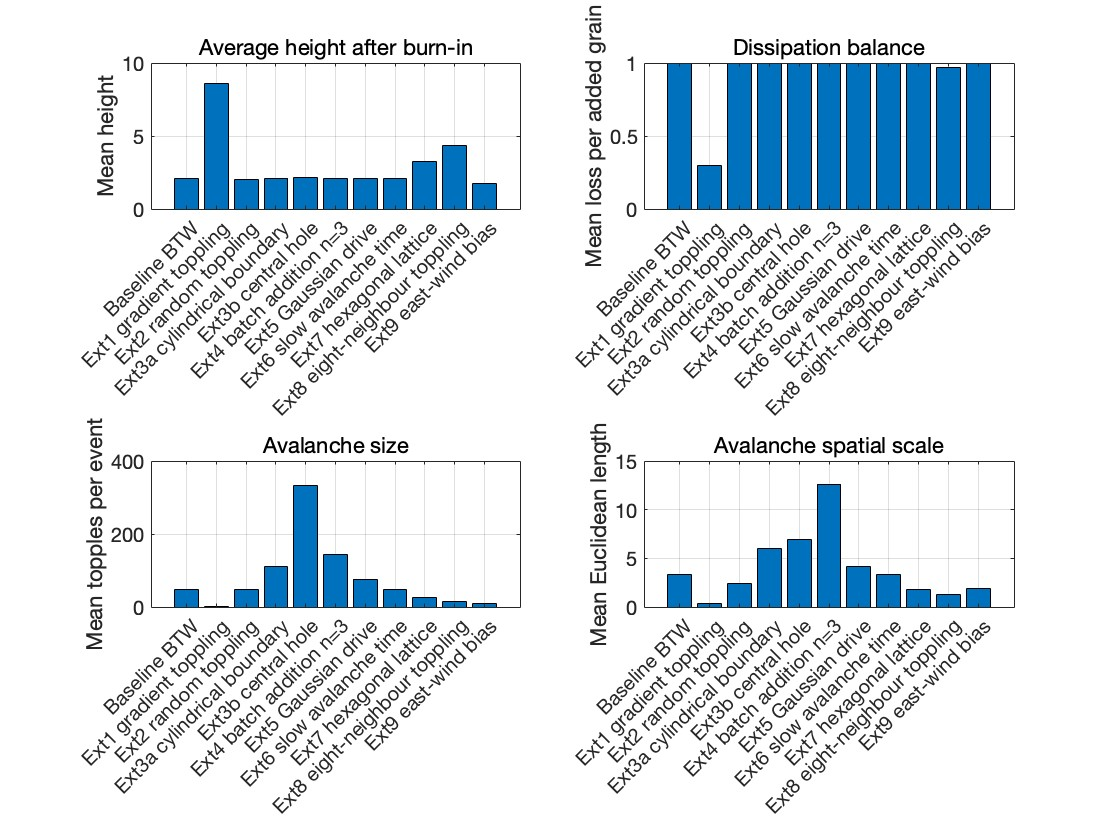
\includegraphics[width=0.7\linewidth]{extend1.jpg}
    \caption{BTW extension summary}
    \label{fig:placeholder}
\end{figure}

\begin{figure}[htbp]
    \centering
    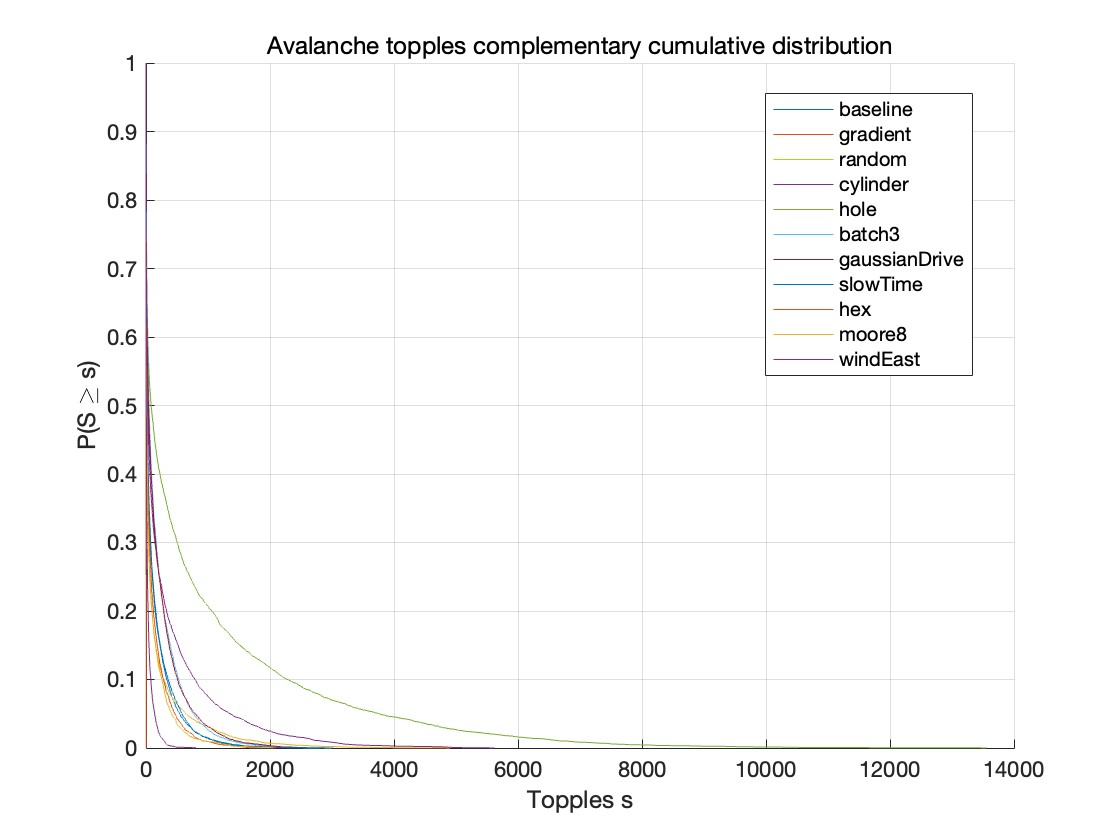
\includegraphics[width=0.7\linewidth]{extend2.jpg}
    \caption{BTW extension topples CCDF}
    \label{fig:placeholder}
\end{figure}

\begin{figure}[htbp]
    \centering
    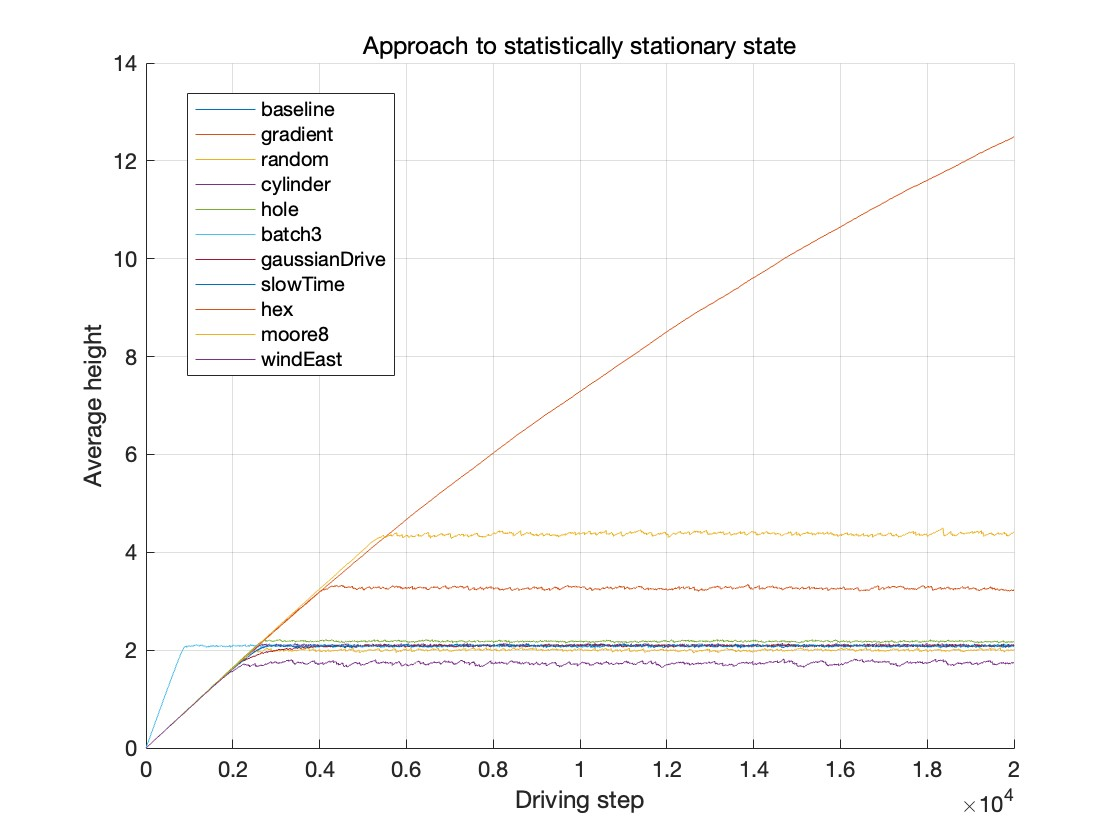
\includegraphics[width=0.7\linewidth]{extend3.jpg}
    \caption{BTW extension height time series}
    \label{fig:placeholder}
\end{figure}

\clearpage

\subsection{Conclusion}

The extensions share the main structure of the BTW model: local instability, relaxation by redistribution, external driving, and dissipation. The main differences are the instability criterion, redistribution rule, boundary geometry, driving protocol, lattice geometry, interaction range, and spatial symmetry. Therefore, the extended models may still show broad avalanche statistics, but they need not have the same height distribution, scaling exponents, cutoff sizes, or spatial correlations as the baseline BTW model.



\clearpage

\section{Reference}


\clearpage


\section{Appendix}
\subsection{Average Height}
In a steady state, a topple occurs when the amount of sand at a certain point reaches 4. Therefore, in a steady state, each height can only be 0, 1, 2, or 3. However, this steady state does not occur with equal probability; that is to say,

$$
P(0) \neq P(1) \neq P(2) \neq P(3)
$$

Once the system reaches a self-organized criticality (SOC) steady state, not all stable configurations appear with equal frequency; rather, the system evolves solely upon so-called "recurrent configurations." Therefore, the average height should be calculated as a weighted average:

$$
<p> = 0 P_0 +P_1+2P_3+3P_3
$$

For the two-dimensional infinite square lattice BTW model, in the steady state, the probabilities that a randomly chosen bulk site has a height of 0, 1, 2, or 3 are, respectively:

\begin{align}
    P_o = \frac{2}{\pi^2} - \frac{4}{\pi^3}\\
    P_1 = \frac{1}{4} - \frac{1}{2\pi}-\frac{3}{\pi^2}+\frac{12}{\pi^3}\\
    P_2 = \frac{3}{8}-\frac{1}{\pi}-\frac{12}{\pi^3}\\
    P_3 = \frac{3}{8}-\frac{1}{2\pi}+\frac{1}{\pi^2}+\frac{4}{\pi^3}
\end{align}

We then have:

\begin{align}
    <p> = 0 \times (\frac{2}{\pi^2} - \frac{4}{\pi^3}) + 1 \times (\frac{1}{4} - \frac{1}{2\pi}-\frac{3}{\pi^2}+\frac{12}
    {\pi^3})+2 \times (\frac{3}{8}-\frac{1}{\pi}-\frac{12}{\pi^3}) +3 \times (\frac{3}{8}-\frac{1}{2\pi}+\frac{1}{\pi^2}+\frac{4}{\pi^3})
\end{align}

\begin{align}
    <p> =\frac{17}{8} = 2.125
\end{align}

\clearpage

\subsection{Average Height Coding}
\begin{lstlisting}
[avgHeight, avalancheSize, rhoSS] = btw_q4_simulation(50, 50, 50000, 1);


function [avgHeight, avalancheSize, rhoSS] = btw_q4_simulation(N, M, nSteps, seed)

    if nargin < 1 || isempty(N)
        N = 50;
    end
    if nargin < 2 || isempty(M)
        M = 50;
    end
    if nargin < 3 || isempty(nSteps)
        nSteps = 50000;
    end
    if nargin < 4 || isempty(seed)
        seed = 1;
    end

    N = floor(N);
    M = floor(M);
    nSteps = floor(nSteps);

    rng(seed);

    pile = zeros(N, M);
    avgHeight = zeros(nSteps, 1);
    avalancheSize = zeros(nSteps, 1);

    for t = 1:nSteps
        % Slow drive: add one grain at a random site
        i = randi(N);
        j = randi(M);
        pile(i, j) = pile(i, j) + 1;

        % Fast relaxation: topple until the configuration is stable
        [pile, avalancheSize(t)] = relaxSandpile(pile);

        % Record average height after full relaxation
        avgHeight(t) = mean(pile(:));
    end

    % Estimate the steady-state average height from the final 20% of the run
    tail = min(nSteps, max(1000, floor(0.2 * nSteps)));
    rhoSS = mean(avgHeight(end - tail + 1:end));

    fprintf('Grid size                        : %d x %d\n', N, M);
    fprintf('Number of grain additions        : %d\n', nSteps);
    fprintf('Estimated steady-state <p_t>     : %.6f\n', rhoSS);
    fprintf('Theoretical large-system limit   : %.6f\n', 17/8);

    % -------- Figure 1: raw average-height trajectory --------
    figure;
    plot(1:nSteps, avgHeight, 'LineWidth', 1.0);
    hold on;
    plot([1, nSteps], [rhoSS, rhoSS], '--', 'LineWidth', 1.2);
    plot([1, nSteps], [17/8, 17/8], '-.', 'LineWidth', 1.2);
    hold off;
    grid on;
    xlabel('Number of grains added');
    ylabel('<p_t>');
    title(sprintf('BTW sandpile on a %d x %d lattice', N, M));
    legend('<p_t>', 'simulated steady-state mean', '17/8 theoretical limit', ...
           'Location', 'best');

    % -------- Figure 2: smoothed trajectory to show saturation more clearly --------
    window = max(100, round(nSteps / 200));
    kernel = ones(window, 1) / window;
    smoothAvg = conv(avgHeight, kernel, 'same');

    figure;
    plot(1:nSteps, smoothAvg, 'LineWidth', 1.5);
    hold on;
    plot([1, nSteps], [rhoSS, rhoSS], '--', 'LineWidth', 1.2);
    hold off;
    grid on;
    xlabel('Number of grains added');
    ylabel(sprintf('moving average of <p_t> (window = %d)', window));
    title('Approach to the stationary state');
    legend('smoothed <p_t>', 'simulated steady-state mean', 'Location', 'best');
end

function [pile, toppleCount] = relaxSandpile(pile)
% RELAXSANDPILE  Fully relax the current lattice.
% The update is done wave-by-wave. For the Abelian sandpile, the final
% stable configuration is independent of toppling order.

    toppleCount = 0;

    while true
        unstable = (pile >= 4);
        if ~any(unstable(:))
            break;
        end

        toppleCount = toppleCount + sum(unstable(:));

        % Each unstable site loses 4 grains
        pile = pile - 4 * unstable;

        % Distribute one grain to each nearest neighbor.
        % Grains that would leave the lattice are simply not added anywhere,
        % which implements open-boundary dissipation.
        pile(2:end, :)   = pile(2:end, :)   + unstable(1:end-1, :); % from above
        pile(1:end-1, :) = pile(1:end-1, :) + unstable(2:end, :);   % from below
        pile(:, 2:end)   = pile(:, 2:end)   + unstable(:, 1:end-1); % from left
        pile(:, 1:end-1) = pile(:, 1:end-1) + unstable(:, 2:end);   % from right
    end
end
\end{lstlisting}

\clearpage

\subsection{Avalanche}
\begin{lstlisting}
clear; 
close all; 
clc;

N = 50;
M = 50;
nSteps = 100000;
burnIn = 20000;
seed = 1;
makePlots = true;

results = btw_avalanche_simulation(N, M, nSteps, burnIn, seed, makePlots);

save('btw_results.mat', 'results');

function results = btw_avalanche_simulation(N, M, nSteps, burnIn, seed, makePlots)

    if nargin < 1 || isempty(N),         N = 50;        end
    if nargin < 2 || isempty(M),         M = N;         end
    if nargin < 3 || isempty(nSteps),    nSteps = 100000; end
    if nargin < 4 || isempty(burnIn),    burnIn = floor(0.2*nSteps); end
    if nargin < 5 || isempty(seed),      seed = 1;      end
    if nargin < 6 || isempty(makePlots), makePlots = true; end

    if burnIn < 0 || burnIn >= nSteps
        error('burnIn must satisfy 0 <= burnIn < nSteps.');
    end

    rng(seed, 'twister');

    pile = zeros(N, M);

    avgHeight = zeros(nSteps, 1);
    topples   = zeros(nSteps, 1);
    area      = zeros(nSteps, 1);
    loss      = zeros(nSteps, 1);
    len       = zeros(nSteps, 1);

    heightCounts = zeros(1, 4);  % counts of stable heights 0,1,2,3 after burnin

    for t = 1:nSteps
        % slow external drive: add one grain at a random site.
        r0 = randi(N);
        c0 = randi(M);
        pile(r0, c0) = pile(r0, c0) + 1;

        % fast internal relaxation: complete the whole avalanche.
        [pile, stats] = relax_avalanche(pile, r0, c0);

        avgHeight(t) = mean(pile(:));
        topples(t)   = stats.topples;
        area(t)      = stats.area;
        loss(t)      = stats.loss;
        len(t)       = stats.length;

        % stable height distribution only after the transient period.
        if t > burnIn
            heightCounts(1) = heightCounts(1) + sum(pile(:) == 0);
            heightCounts(2) = heightCounts(2) + sum(pile(:) == 1);
            heightCounts(3) = heightCounts(3) + sum(pile(:) == 2);
            heightCounts(4) = heightCounts(4) + sum(pile(:) == 3);
        end
    end

    steadyIdx = (burnIn+1):nSteps;
    avalancheIdx = steadyIdx(topples(steadyIdx) > 0);

    results = struct();
    results.N = N;
    results.M = M;
    results.nSteps = nSteps;
    results.burnIn = burnIn;
    results.seed = seed;
    results.finalPile = pile;
    results.avgHeight = avgHeight;
    results.topples = topples;
    results.area = area;
    results.loss = loss;
    results.length = len;
    results.meanHeightAfterBurnIn = mean(avgHeight(steadyIdx));
    results.meanLossPerAddedGrainAfterBurnIn = mean(loss(steadyIdx));
    results.fractionNonzeroAvalanchesAfterBurnIn = numel(avalancheIdx) / numel(steadyIdx);
    results.heightProbabilityAfterBurnIn = heightCounts / sum(heightCounts);

    % data restricted to nonzero avalanches after burn-in.
    avalancheTopples = topples(avalancheIdx);
    avalancheArea    = area(avalancheIdx);
    avalancheLoss    = loss(avalancheIdx);
    avalancheLength  = len(avalancheIdx);

    results.avalancheTopples = avalancheTopples;
    results.avalancheArea = avalancheArea;
    results.avalancheLoss = avalancheLoss;
    results.avalancheLength = avalancheLength;
    results.zeroLossFractionAmongAvalanches = mean(avalancheLoss == 0);

    % power-law fits from log-binned empirical PDFs.
    % these are rough estimates; choose the fitted range manually for a final report.
    nBins = 25;
    results.fitTopples = log_binned_powerlaw_fit(avalancheTopples, nBins);
    results.fitArea    = log_binned_powerlaw_fit(avalancheArea, nBins);
    results.fitLength  = log_binned_powerlaw_fit(avalancheLength, nBins);
    results.fitLossPositive = log_binned_powerlaw_fit(avalancheLoss(avalancheLoss > 0), nBins);

    % Correlation between avalanche observables.
    % Use log(1+x) because the distributions are heavy-tailed.
    if numel(avalancheTopples) >= 2
        X = [avalancheTopples, avalancheArea, avalancheLoss, avalancheLength];
        results.correlationLog1p = corrcoef(log(1 + X));
    else
        results.correlationLog1p = NaN(4,4);
    end

    print_summary(results);

    if makePlots
        make_btw_plots(results);
    end
end

function [pile, stats] = relax_avalanche(pile, r0, c0)
%RELAX_AVALANCHE Relax one avalanche using a queue of unstable sites.

    [N, M] = size(pile);

    stats = struct('topples', 0, 'area', 0, 'loss', 0, 'length', 0);
    toppledMask = false(N, M);

    queue = zeros(1024, 1);
    head = 1;
    tail = 0;

    originIdx = sub2ind([N, M], r0, c0);
    if pile(originIdx) >= 4
        [queue, tail] = push_queue(queue, tail, originIdx);
    end

    dr = [-1, 1, 0, 0];
    dc = [0, 0, -1, 1];

    while head <= tail
        idx = queue(head);
        head = head + 1;

        % Duplicate entries in the queue are allowed; skip if already stable.
        if pile(idx) < 4
            continue;
        end

        [r, c] = ind2sub([N, M], idx);

        pile(idx) = pile(idx) - 4;
        stats.topples = stats.topples + 1;
        toppledMask(idx) = true;

        % If the same site is still unstable, queue it again.
        if pile(idx) >= 4
            [queue, tail] = push_queue(queue, tail, idx);
        end

        % Send one grain to each nearest neighbour, or lose it at the boundary.
        for k = 1:4
            rn = r + dr(k);
            cn = c + dc(k);

            if rn >= 1 && rn <= N && cn >= 1 && cn <= M
                nIdx = sub2ind([N, M], rn, cn);
                pile(nIdx) = pile(nIdx) + 1;
                if pile(nIdx) >= 4
                    [queue, tail] = push_queue(queue, tail, nIdx);
                end
            else
                stats.loss = stats.loss + 1;
            end
        end
    end

    stats.area = sum(toppledMask(:));

    if stats.area > 0
        [rr, cc] = find(toppledMask);
        stats.length = max(sqrt((rr - r0).^2 + (cc - c0).^2));
    else
        stats.length = 0;
    end
end

function [queue, tail] = push_queue(queue, tail, idx)
    tail = tail + 1;
    if tail > numel(queue)
        queue = [queue; zeros(max(1024, numel(queue)), 1)]; %#ok<AGROW>
    end
    queue(tail) = idx;
end

function fit = log_binned_powerlaw_fit(x, nBins)
%This is a simple diagnostic fit, not a full maximum-likelihood power-law test.

    x = x(:);
    x = x(isfinite(x) & x > 0);

    fit = struct();
    fit.tau = NaN;
    fit.slope = NaN;
    fit.intercept = NaN;
    fit.centers = [];
    fit.pdf = [];
    fit.fitCenters = [];
    fit.fitPdf = [];
    fit.n = numel(x);

    if numel(x) < 20 || numel(unique(x)) < 3
        return;
    end

    xmin = min(x);
    xmax = max(x);

    if xmin <= 0 || xmax <= xmin
        return;
    end

    edges = logspace(log10(xmin), log10(xmax), nBins + 1);
    edges = unique(edges);

    if numel(edges) < 4
        return;
    end

    counts = histcounts(x, edges);
    widths = diff(edges);
    centers = sqrt(edges(1:end-1) .* edges(2:end));
    pdf = counts ./ (sum(counts) .* widths);

    valid = counts > 0 & pdf > 0 & isfinite(pdf);
    validIdx = find(valid);

    if numel(validIdx) < 3
        fit.centers = centers(valid);
        fit.pdf = pdf(valid);
        return;
    end

    % scaling region manually.
    if numel(validIdx) >= 7
        fitIdx = validIdx(2:end-1);
    else
        fitIdx = validIdx;
    end

    logx = log10(centers(fitIdx));
    logy = log10(pdf(fitIdx));
    p = polyfit(logx, logy, 1);

    fit.slope = p(1);
    fit.intercept = p(2);
    fit.tau = -p(1);
    fit.centers = centers(valid);
    fit.pdf = pdf(valid);
    fit.fitCenters = centers(fitIdx);
    fit.fitPdf = 10.^(polyval(p, log10(centers(fitIdx))));
end

function print_summary(results)
%summary

    fprintf('\n===== BTW sandpile simulation summary =====\n');
    fprintf('Lattice size: %d x %d\n', results.N, results.M);
    fprintf('Steps: %d, burn-in: %d\n', results.nSteps, results.burnIn);
    fprintf('Mean height after burn-in: %.6f\n', results.meanHeightAfterBurnIn);
    fprintf('Reference infinite-lattice value for this height convention: 17/8 = %.6f\n', 17/8);
    fprintf('Mean loss per added grain after burn-in: %.6f\n', results.meanLossPerAddedGrainAfterBurnIn);
    fprintf('Fraction of nonzero avalanches after burn-in: %.6f\n', results.fractionNonzeroAvalanchesAfterBurnIn);

    hp = results.heightProbabilityAfterBurnIn;
    fprintf('Height probabilities after burn-in: P(0)=%.4f, P(1)=%.4f, P(2)=%.4f, P(3)=%.4f\n', hp(1), hp(2), hp(3), hp(4));

    fprintf('\nApproximate log-binned power-law exponents P(x) ~ x^{-tau}:\n');
    fprintf('  topples tau  = %.4f\n', results.fitTopples.tau);
    fprintf('  area tau     = %.4f\n', results.fitArea.tau);
    fprintf('  length tau   = %.4f\n', results.fitLength.tau);
    fprintf('  positive loss tau = %.4f\n', results.fitLossPositive.tau);
    fprintf('  fraction of avalanches with zero loss = %.4f\n', results.zeroLossFractionAmongAvalanches);

    fprintf('\nCorrelation matrix of log(1+x) for [topples, area, loss, length]:\n');
    disp(results.correlationLog1p);
    fprintf('===========================================\n\n');
end

function make_btw_plots(results)
%Pot
    nSteps = results.nSteps;
    burnIn = results.burnIn;
    t = (1:nSteps).';

    figure;
    plot(t, results.avgHeight);
    hold on;
    plot([burnIn burnIn], ylim, '--');
    plot([1 nSteps], [results.meanHeightAfterBurnIn results.meanHeightAfterBurnIn], '--');
    plot([1 nSteps], [17/8 17/8], ':');
    xlabel('external time step');
    ylabel('mean height <p_t>');
    title('Mean sandpile height');
    legend('simulation', 'burn-in', 'post-burn-in mean', '17/8 reference', 'Location', 'best');
    grid on;

    figure;
    bar(0:3, results.heightProbabilityAfterBurnIn);
    xlabel('stable site height');
    ylabel('probability');
    title('Height distribution after burn-in');
    grid on;

    plot_fit(results.fitTopples, 'Topples', 's');
    plot_fit(results.fitArea, 'Area', 'a');
    plot_fit(results.fitLength, 'Euclidean length', 'ell');
    plot_fit(results.fitLossPositive, 'Positive loss', 'loss');

    figure;
    imagesc(results.correlationLog1p, [-1 1]);
    colorbar;
    axis square;
    set(gca, 'XTick', 1:4, 'YTick', 1:4);
    set(gca, 'XTickLabel', {'topples','area','loss','length'});
    set(gca, 'YTickLabel', {'topples','area','loss','length'});
    title('Correlation of log(1+x) avalanche observables');
end

function plot_fit(fit, plotTitle, symbolName)
%Plot a log-binned empirical PDF and the fitted power-law region.

    figure;

    if isempty(fit.centers)
        text(0.1, 0.5, 'Not enough data to plot.');
        title(plotTitle);
        return;
    end

    loglog(fit.centers, fit.pdf, 'o');
    hold on;

    if ~isempty(fit.fitCenters) && all(isfinite(fit.fitPdf))
        loglog(fit.fitCenters, fit.fitPdf, '-');
        legend('log-binned empirical PDF', sprintf('fit: tau = %.3f', fit.tau), 'Location', 'best');
    else
        legend('log-binned empirical PDF', 'Location', 'best');
    end

    xlabel(symbolName);
    ylabel(sprintf('P(%s)', symbolName));
    title(plotTitle);
    grid on;
end
\end{lstlisting}


\clearpage

\subsection{abelian btw}

\begin{lstlisting}
function results = verify_abelian_btw(nTrials, N, M, nExtraGrains, rngSeed)

    if nargin < 1 || isempty(nTrials),     nTrials = 200; end
    if nargin < 2 || isempty(N),           N = 20; end
    if nargin < 3 || isempty(M),           M = N; end
    if nargin < 4 || isempty(nExtraGrains), nExtraGrains = 80; end
    if nargin < 5 || isempty(rngSeed),     rngSeed = 1; end

    rng(rngSeed);

    fprintf('\n=== BTW Abelian-property check ===\n');

    %% the 3-by-3 example
    S0 = [2 3 1; 1 4 0; 2 3 2];
    stats0 = make_stats(3, 3);
    [S1, ~] = topple_site(S0, 2, 2, stats0);

    statsA = make_stats(3, 3);
    [SA, statsA] = topple_site(S1, 1, 2, statsA);  % topple upper unstable site first
    [SA, statsA] = topple_site(SA, 3, 2, statsA);  % then lower unstable site

    statsB = make_stats(3, 3);
    [SB, statsB] = topple_site(S1, 3, 2, statsB);  % topple lower unstable site first
    [SB, statsB] = topple_site(SB, 1, 2, statsB);  % then upper unstable site

    fprintf('\nInitial configuration:\n');
    disp(S0);
    fprintf('After toppling the centre site:\n');
    disp(S1);
    fprintf('Final state: upper site then lower site:\n');
    disp(SA);
    fprintf('Final state: lower site then upper site:\n');
    disp(SB);

    assert(isequal(SA, SB), 'The two explicit orders did not give the same final state.');
    fprintf('The two orders give the same final configuration.\n');

    %% random tests
    allSameFinal = true;
    allSameOdometer = true;
    allSameLoss = true;
    firstFailure = struct('trial', [], 'kind', '');

    for trial = 1:nTrials
        pile0 = randi([0, 3], N, M);

        % Add a finite number of extra grains to create unstable sites.
        for k = 1:nExtraGrains
            r = randi(N);
            c = randi(M);
            pile0(r, c) = pile0(r, c) + 1;
        end

        [pFirst, sFirst]   = relax_order(pile0, 'first',  rngSeed + trial);
        [pLast, sLast]     = relax_order(pile0, 'last',   rngSeed + trial);
        [pRandom, sRandom] = relax_order(pile0, 'random', rngSeed + trial);

        sameFinal = isequal(pFirst, pLast) && isequal(pFirst, pRandom);
        sameOdometer = isequal(sFirst.toppleCounts, sLast.toppleCounts) && ...
                       isequal(sFirst.toppleCounts, sRandom.toppleCounts);
        sameLoss = (sFirst.loss == sLast.loss) && (sFirst.loss == sRandom.loss);

        if ~sameFinal && allSameFinal
            firstFailure.trial = trial;
            firstFailure.kind = 'final configuration';
        end
        if ~sameOdometer && allSameOdometer
            firstFailure.trial = trial;
            firstFailure.kind = 'topple-count matrix';
        end
        if ~sameLoss && allSameLoss
            firstFailure.trial = trial;
            firstFailure.kind = 'loss';
        end

        allSameFinal = allSameFinal && sameFinal;
        allSameOdometer = allSameOdometer && sameOdometer;
        allSameLoss = allSameLoss && sameLoss;

        if ~(allSameFinal && allSameOdometer && allSameLoss)
            break;
        end
    end

    fprintf('\nRandom tests: %d trial(s) on %d-by-%d lattices with %d extra grains.\n', ...
            nTrials, N, M, nExtraGrains);
    fprintf('Same final stable configuration for all tested orders: %d\n', allSameFinal);
    fprintf('Same toppling-count matrix for all tested orders:       %d\n', allSameOdometer);
    fprintf('Same boundary loss for all tested orders:              %d\n', allSameLoss);

    if allSameFinal && allSameOdometer && allSameLoss
        fprintf('All tests passed. This numerically verifies the Abelian property.\n');
    else
        fprintf('First failure: trial %d, quantity: %s.\n', firstFailure.trial, firstFailure.kind);
    end

    results.example.initial = S0;
    results.example.afterCentreTopple = S1;
    results.example.finalUpperThenLower = SA;
    results.example.finalLowerThenUpper = SB;
    results.randomTests.nTrials = nTrials;
    results.randomTests.N = N;
    results.randomTests.M = M;
    results.randomTests.nExtraGrains = nExtraGrains;
    results.randomTests.sameFinal = allSameFinal;
    results.randomTests.sameOdometer = allSameOdometer;
    results.randomTests.sameLoss = allSameLoss;
end

function [pile, stats] = relax_order(pile, orderMode, rngSeed)
%RELAX_ORDER Stabilize a sandpile using a specified legal toppling order.
% orderMode = 'first', 'last', or 'random'.

    if nargin >= 3 && ~isempty(rngSeed)
        rng(rngSeed);
    end

    [N, M] = size(pile);
    stats = make_stats(N, M);
    maxTopples = 1e7;  % safety guard against accidental infinite loops

    while true
        unstable = find(pile >= 4);
        if isempty(unstable)
            break;
        end

        switch lower(orderMode)
            case 'first'
                siteIndex = unstable(1);
            case 'last'
                siteIndex = unstable(end);
            case 'random'
                siteIndex = unstable(randi(numel(unstable)));
            otherwise
                error('Unknown orderMode. Use ''first'', ''last'', or ''random''.');
        end

        [r, c] = ind2sub([N, M], siteIndex);
        [pile, stats] = topple_site(pile, r, c, stats);

        if stats.totalTopples > maxTopples
            error('Exceeded maxTopples. Check the input configuration.');
        end
    end

    stats.area = nnz(stats.toppleCounts > 0);
end

function [pile, stats] = topple_site(pile, r, c, stats)
%Topple site (r,c) once using open-boundary BTW rules.

    [N, M] = size(pile);

    pile(r, c) = pile(r, c) - 4;
    stats.totalTopples = stats.totalTopples + 1;
    stats.toppleCounts(r, c) = stats.toppleCounts(r, c) + 1;

    neighbours = [r-1, c; r+1, c; r, c-1; r, c+1];
    for q = 1:4
        rr = neighbours(q, 1);
        cc = neighbours(q, 2);

        if rr >= 1 && rr <= N && cc >= 1 && cc <= M
            pile(rr, cc) = pile(rr, cc) + 1;
        else
            stats.loss = stats.loss + 1;
        end
    end
end

function stats = make_stats(N, M)
%MAKE_STATS Initialize counters for a relaxation.

    stats.totalTopples = 0;
    stats.loss = 0;
    stats.toppleCounts = zeros(N, M);
    stats.area = 0;
end
\end{lstlisting}

\clearpage

\subsection{btw toppling matrix}
\begin{lstlisting}
function results = btw_toppling_matrix_demo_v2(nTrials, N, M, maxExtraGrains, rngSeed)

    if nargin < 1 || isempty(nTrials),       nTrials = 200; end
    if nargin < 2 || isempty(N),             N = 20; end
    if nargin < 3 || isempty(M),             M = 20; end
    if nargin < 4 || isempty(maxExtraGrains),maxExtraGrains = 80; end
    if nargin < 5 || isempty(rngSeed),       rngSeed = 1; end

    rng(rngSeed);
    k = 4; % 2d for d = 2

    fprintf('\n=== BTW toppling-matrix and Abelian-property demo ===\n');
    fprintf('Lattice size for random tests: %d-by-%d\n', N, M);
    fprintf('Number of random trials:       %d\n\n', nTrials);

    %% build and check the toppling matrix Delta.
    Delta = buildDelta2D(N, M);
    nSites = N * M;

    offDiag = Delta - spdiags(diag(Delta), 0, nSites, nSites);
    rowSums = full(sum(Delta, 2));

    % convert all logical checks to ordinary full scalar logicals.
    cond4a = logical(isequal(Delta, Delta.') && all(full(nonzeros(offDiag)) >= 0));
    cond4b = logical(full(all(full(diag(Delta)) < 0)));
    cond4c = logical(full(all(rowSums <= 0)));
    cond4d = logical(full(sum(Delta(:))) < 0);

    fprintf('Eq. (4a), off-diagonal symmetry and non-negativity: %d\n', double(cond4a));
    fprintf('Eq. (4b), negative diagonal entries:                %d\n', double(cond4b));
    fprintf('Eq. (4c), non-positive row sums:                    %d\n', double(cond4c));
    fprintf('Eq. (4d), strictly negative total sum:              %d\n', double(cond4d));
    fprintf('Stability threshold k = -Delta(x,x) = %d in 2D.\n\n', -full(Delta(1,1)));

    %% 2. reproduce the 3-by-3 example from the notes.
    p0 = [2 3 1; 1 4 0; 2 3 2];
    p1 = toppleOnce(p0, 2, 2, k);       % topple the central site
    pUpperThenLower = toppleOnce(toppleOnce(p1, 1, 2, k), 3, 2, k);
    pLowerThenUpper = toppleOnce(toppleOnce(p1, 3, 2, k), 1, 2, k);

    fprintf('3-by-3 example from the notes:\n');
    fprintf('Initial configuration p0:\n'); disp(p0);
    fprintf('After toppling the centre site:\n'); disp(p1);
    fprintf('Final state, upper then lower:\n'); disp(pUpperThenLower);
    fprintf('Final state, lower then upper:\n'); disp(pLowerThenUpper);
    fprintf('The two final states are identical: %d\n\n', double(isequal(pUpperThenLower, pLowerThenUpper)));

    %% 3. random commutation tests for two legal topplings.
    sameTwoToppleOrder = true;
    for trial = 1:nTrials
        pile = randi([0, k-1], N, M);
        x = randi(N*M);
        y = randi(N*M);
        while y == x
            y = randi(N*M);
        end
        [rx, cx] = ind2sub([N, M], x);
        [ry, cy] = ind2sub([N, M], y);

        % Force both chosen sites to be unstable initially.
        pile(rx, cx) = k + randi([0, 3]);
        pile(ry, cy) = k + randi([0, 3]);

        pxy = toppleOnce(toppleOnce(pile, rx, cx, k), ry, cy, k);
        pyx = toppleOnce(toppleOnce(pile, ry, cy, k), rx, cx, k);

        if ~isequal(pxy, pyx)
            sameTwoToppleOrder = false;
            break;
        end
    end
    fprintf('Random two-toppling commutation tests passed:       %d\n', double(sameTwoToppleOrder));

    %% 4. random stabilization tests using different legal toppling orders.
    sameFinalState = true;
    sameToppleCounts = true;
    sameLoss = true;

    for trial = 1:nTrials
        % Start from a stable pile, then add a finite number of extra grains.
        pile0 = randi([0, k-1], N, M);
        nExtra = randi(maxExtraGrains);
        for g = 1:nExtra
            r = randi(N);
            c = randi(M);
            pile0(r, c) = pile0(r, c) + 1;
        end

        [pFirst, uFirst, lossFirst] = stabilize(pile0, 'first',  k);
        [pLast,  uLast,  lossLast]  = stabilize(pile0, 'last',   k);
        [pRand,  uRand,  lossRand]  = stabilize(pile0, 'random', k);

        if ~(isequal(pFirst, pLast) && isequal(pFirst, pRand))
            sameFinalState = false;
            break;
        end
        if ~(isequal(uFirst, uLast) && isequal(uFirst, uRand))
            sameToppleCounts = false;
            break;
        end
        if ~(lossFirst == lossLast && lossFirst == lossRand)
            sameLoss = false;
            break;
        end
    end

    fprintf('Random stabilization tests, same final state:       %d\n', double(sameFinalState));
    fprintf('Random stabilization tests, same topple counts:     %d\n', double(sameToppleCounts));
    fprintf('Random stabilization tests, same boundary loss:     %d\n\n', double(sameLoss));

    if cond4a && cond4b && cond4c && cond4d && sameTwoToppleOrder && sameFinalState && sameToppleCounts && sameLoss
        fprintf('All checks passed. This numerically supports the Abelian property.\n');
    else
        fprintf('At least one check failed. Inspect the returned results.\n');
    end

    results = struct();
    results.Delta = Delta;
    results.k = k;
    results.conditions = struct('cond4a', cond4a, 'cond4b', cond4b, 'cond4c', cond4c, 'cond4d', cond4d);
    results.example = struct('p0', p0, 'afterCentreTopple', p1, ...
        'upperThenLower', pUpperThenLower, 'lowerThenUpper', pLowerThenUpper);
    results.tests = struct('sameTwoToppleOrder', sameTwoToppleOrder, ...
        'sameFinalState', sameFinalState, 'sameToppleCounts', sameToppleCounts, 'sameLoss', sameLoss);
end

function Delta = buildDelta2D(N, M)
    nSites = N * M;
    Delta = spalloc(nSites, nSites, 5*nSites);
    for r = 1:N
        for c = 1:M
            x = sub2ind([N, M], r, c);
            Delta(x, x) = -4;
            if r > 1
                y = sub2ind([N, M], r-1, c);
                Delta(x, y) = 1;
            end
            if r < N
                y = sub2ind([N, M], r+1, c);
                Delta(x, y) = 1;
            end
            if c > 1
                y = sub2ind([N, M], r, c-1);
                Delta(x, y) = 1;
            end
            if c < M
                y = sub2ind([N, M], r, c+1);
                Delta(x, y) = 1;
            end
        end
    end
end

function pile = toppleOnce(pile, r, c, k)
    % apply one legal or algebraic toppling at site (r,c).
    % the caller is responsible for using it legally in the BTW dynamics.
    [N, M] = size(pile);
    pile(r, c) = pile(r, c) - k;
    if r > 1, pile(r-1, c) = pile(r-1, c) + 1; end
    if r < N, pile(r+1, c) = pile(r+1, c) + 1; end
    if c > 1, pile(r, c-1) = pile(r, c-1) + 1; end
    if c < M, pile(r, c+1) = pile(r, c+1) + 1; end
end

function [pile, toppleCounts, loss] = stabilize(pile, mode, k)
    [N, M] = size(pile);
    toppleCounts = zeros(N, M);
    loss = 0;
    maxTopples = 1e7;
    nTopples = 0;

    while true
        unstable = find(pile >= k);
        if isempty(unstable)
            break;
        end

        switch lower(mode)
            case 'first'
                idx = unstable(1);
            case 'last'
                idx = unstable(end);
            case 'random'
                idx = unstable(randi(numel(unstable)));
            otherwise
                error('Unknown mode: %s', mode);
        end

        [r, c] = ind2sub([N, M], idx);
        [pile, lostNow] = legalToppleWithLoss(pile, r, c, k);
        toppleCounts(r, c) = toppleCounts(r, c) + 1;
        loss = loss + lostNow;
        nTopples = nTopples + 1;

        if nTopples > maxTopples
            error('Exceeded maxTopples. Something is probably wrong.');
        end
    end
end

function [pile, lost] = legalToppleWithLoss(pile, r, c, k)
    [N, M] = size(pile);
    lost = 0;

    pile(r, c) = pile(r, c) - k;

    if r > 1
        pile(r-1, c) = pile(r-1, c) + 1;
    else
        lost = lost + 1;
    end

    if r < N
        pile(r+1, c) = pile(r+1, c) + 1;
    else
        lost = lost + 1;
    end

    if c > 1
        pile(r, c-1) = pile(r, c-1) + 1;
    else
        lost = lost + 1;
    end

    if c < M
        pile(r, c+1) = pile(r, c+1) + 1;
    else
        lost = lost + 1;
    end
end
\end{lstlisting}

\clearpage

\subsection{Extension}
\begin{lstlisting}
function [summary, allResults] = btw_extensions_simulation(models, opts)

    if nargin < 1 || isempty(models)
        models = default_extension_models();
    end
    if nargin < 2
        opts = struct();
    end
    opts = fill_default_opts(opts);

    nModels = numel(models);
    allResults = cell(nModels, 1);

    fprintf('\n=== BTW extension comparison ===\n');
    fprintf('Lattice: %d-by-%d, steps: %d, burn-in: %d\n', ...
        opts.N, opts.M, opts.nSteps, opts.burnIn);
    fprintf('Number of model variants including baseline: %d\n\n', nModels);

    for m = 1:nModels
        fprintf('[%2d/%2d] Running %s ...\n', m, nModels, models(m).name);
        if opts.sameSeedForAll
            rng(opts.seed, 'twister');
        else
            rng(opts.seed + 1009*(m-1), 'twister');
        end
        allResults{m} = simulate_one_model(models(m), opts);
    end

    summary = build_summary_table(allResults, opts);
    disp(summary);

    if opts.saveTable
        try
            writetable(summary, opts.summaryCsvName);
            fprintf('Summary table written to %s\n', opts.summaryCsvName);
        catch ME
            warning('Could not write summary table: %s', ME.message);
        end
    end

    if opts.makePlots
        plot_comparison(allResults, summary, opts);
    end

    if opts.saveMat
        try
            save(opts.matFileName, 'summary', 'allResults', 'opts', 'models');
            fprintf('Results saved to %s\n', opts.matFileName);
        catch ME
            warning('Could not save MAT file: %s', ME.message);
        end
    end
end

% -------------------------------------------------------------------------
function opts = fill_default_opts(opts)
    opts = set_default(opts, 'N', 35);
    opts = set_default(opts, 'M', 35);
    opts = set_default(opts, 'nSteps', 20000);
    opts = set_default(opts, 'burnIn', 5000);
    opts = set_default(opts, 'seed', 1);
    opts = set_default(opts, 'sameSeedForAll', false);
    opts = set_default(opts, 'makePlots', true);
    opts = set_default(opts, 'saveFigures', true);
    opts = set_default(opts, 'saveTable', true);
    opts = set_default(opts, 'saveMat', true);
    opts = set_default(opts, 'summaryCsvName', 'btw_extension_summary.csv');
    opts = set_default(opts, 'matFileName', 'btw_extension_results.mat');
    opts = set_default(opts, 'maxRelaxSteps', 500000);
    opts = set_default(opts, 'minFitSamples', 100);
end

function s = set_default(s, fieldName, value)
    if ~isfield(s, fieldName) || isempty(s.(fieldName))
        s.(fieldName) = value;
    end
end

% -------------------------------------------------------------------------
function models = default_extension_models()
    models = repmat(base_model(), 0, 1);

    m = base_model();
    m.name = 'Baseline BTW';
    m.shortName = 'baseline';
    models(end+1) = m;

    % 1. Gradient-dependent toppling.
    m = base_model();
    m.name = 'Ext1 gradient toppling';
    m.shortName = 'gradient';
    m.relaxation = 'gradient';
    m.gradientK = 4;
    models(end+1) = m;

    % 2. Random redistribution of the four grains.
    m = base_model();
    m.name = 'Ext2 random toppling';
    m.shortName = 'random';
    m.redistribution = 'random';
    models(end+1) = m;

    % 3a. Cylindrical boundary: wrap in x/columns, dissipate at top/bottom.
    m = base_model();
    m.name = 'Ext3a cylindrical boundary';
    m.shortName = 'cylinder';
    m.boundary = 'cylinderX';
    models(end+1) = m;

    % 3b. No outer-edge loss; central hole is the sink.
    m = base_model();
    m.name = 'Ext3b central hole';
    m.shortName = 'hole';
    m.boundary = 'reflectOuterHole';
    m.centralHole = true;
    m.holeRadius = 2;
    models(end+1) = m;

    % 4. Faster drive: add multiple grains before relaxation.
    m = base_model();
    m.name = 'Ext4 batch addition n=3';
    m.shortName = 'batch3';
    m.batchN = 3;
    m.batchMode = 'different';
    models(end+1) = m;

    % 5. Non-uniform drive: Gaussian centred on the grid.
    m = base_model();
    m.name = 'Ext5 Gaussian drive';
    m.shortName = 'gaussianDrive';
    m.driveMode = 'gaussian';
    m.driveSigmaFraction = 0.18;
    models(end+1) = m;

    % 6. Slow avalanche interpretation: each topple has a time cost.
    m = base_model();
    m.name = 'Ext6 slow avalanche time';
    m.shortName = 'slowTime';
    m.slowAvalanche = true;
    models(end+1) = m;

    % 7. Hexagonal lattice: six neighbours, threshold six.
    m = base_model();
    m.name = 'Ext7 hexagonal lattice';
    m.shortName = 'hex';
    m.neighbourhood = 'hex';
    m.threshold = 6;
    models(end+1) = m;

    % 8. Eight surrounding sites: Moore neighbourhood, threshold eight.
    m = base_model();
    m.name = 'Ext8 eight-neighbour toppling';
    m.shortName = 'moore8';
    m.neighbourhood = 'moore8';
    m.threshold = 8;
    models(end+1) = m;

    % 9. Wind/slope: biased random transport to the east.
    m = base_model();
    m.name = 'Ext9 east-wind bias';
    m.shortName = 'windEast';
    m.redistribution = 'wind';
    % Offset order for von Neumann neighbourhood is [N; E; S; W].
    m.windWeights = [0.15, 0.55, 0.15, 0.10];
    models(end+1) = m;
end

function m = base_model()
    m.name = 'Baseline BTW';
    m.shortName = 'baseline';
    m.relaxation = 'standard';       % 'standard' or 'gradient'
    m.neighbourhood = 'vonNeumann';  % 'vonNeumann', 'hex', 'moore8', 'radius2'
    m.threshold = [];                % empty -> number of neighbours
    m.redistribution = 'deterministic'; % deterministic/random/randomWeighted/wind
    m.boundary = 'open';             % open/cylinderX/reflectOuterHole
    m.centralHole = false;
    m.holeRadius = 0;
    m.batchN = 1;
    m.batchMode = 'different';       % same/different
    m.driveMode = 'uniform';         % uniform/gaussian/subset
    m.driveSigmaFraction = 0.18;
    m.subsetFraction = 0.25;
    m.gradientK = 4;
    m.slowAvalanche = false;
    m.windWeights = [0.25, 0.25, 0.25, 0.25];
end

% -------------------------------------------------------------------------
function res = simulate_one_model(model, opts)
    N = opts.N;
    M = opts.M;
    pile = zeros(N, M);
    active = make_active_mask(model, N, M);
    drive = make_drive_distribution(model, active, N, M);

    avgHeight = zeros(opts.nSteps, 1);
    topples = zeros(opts.nSteps, 1);
    area = zeros(opts.nSteps, 1);
    loss = zeros(opts.nSteps, 1);
    len = zeros(opts.nSteps, 1);
    duration = zeros(opts.nSteps, 1);

    for t = 1:opts.nSteps
        [addRows, addCols] = choose_addition_sites(model, drive, active);
        for g = 1:numel(addRows)
            pile(addRows(g), addCols(g)) = pile(addRows(g), addCols(g)) + 1;
        end

        if strcmp(model.relaxation, 'gradient')
            [pile, stats] = relax_gradient(pile, active, model, opts);
        else
            [pile, stats] = relax_standard(pile, active, model, opts);
        end

        avgHeight(t) = mean(pile(active));
        topples(t) = stats.topples;
        area(t) = stats.area;
        loss(t) = stats.loss;
        len(t) = stats.length;
        if model.slowAvalanche
            duration(t) = stats.topples;
        else
            duration(t) = double(stats.topples > 0);
        end
    end

    idx = (opts.burnIn + 1):opts.nSteps;
    if isempty(idx)
        idx = 1:opts.nSteps;
    end

    res.model = model;
    res.active = active;
    res.finalPile = pile;
    res.avgHeight = avgHeight;
    res.topples = topples;
    res.area = area;
    res.loss = loss;
    res.length = len;
    res.duration = duration;
    res.afterBurnIn = idx;

    res.meanHeight = mean(avgHeight(idx));
    res.meanLossPerStep = mean(loss(idx));
    res.meanLossPerGrain = mean(loss(idx)) / model.batchN;
    res.meanTopples = mean(topples(idx));
    res.meanArea = mean(area(idx));
    res.meanLength = mean(len(idx));
    res.meanDuration = mean(duration(idx));
    res.nonzeroAvalancheRate = mean(topples(idx) > 0);

    maxH = max(3, max(pile(active)));
    counts = zeros(maxH + 1, 1);
    vals = pile(active);
    for h = 0:maxH
        counts(h+1) = sum(vals == h);
    end
    res.heightValues = (0:maxH).';
    res.heightProb = counts / sum(active(:));

    res.fitTopplesTau = estimate_power_law_tau(topples(idx), opts.minFitSamples);
    res.fitAreaTau = estimate_power_law_tau(area(idx), opts.minFitSamples);
    res.fitLengthTau = estimate_power_law_tau(len(idx), opts.minFitSamples);
    res.fitPositiveLossTau = estimate_power_law_tau(loss(idx), opts.minFitSamples);

    X = [topples(idx), area(idx), loss(idx), len(idx)];
    X = log1p(X);
    if size(X, 1) > 2 && all(std(X, 0, 1) > 0)
        res.corrLog = corrcoef(X);
    else
        res.corrLog = NaN(4, 4);
    end
end

% -------------------------------------------------------------------------
function active = make_active_mask(model, N, M)
    active = true(N, M);
    if model.centralHole
        [rr, cc] = ndgrid(1:N, 1:M);
        cr = (N + 1) / 2;
        cc0 = (M + 1) / 2;
        hole = (rr - cr).^2 + (cc - cc0).^2 <= model.holeRadius^2;
        active(hole) = false;
    end
end

function drive = make_drive_distribution(model, active, N, M)
    drive.activeLinear = find(active);
    drive.weights = ones(size(drive.activeLinear));

    if strcmp(model.driveMode, 'gaussian')
        [rr, cc] = ndgrid(1:N, 1:M);
        cr = (N + 1) / 2;
        cc0 = (M + 1) / 2;
        sigma = model.driveSigmaFraction * min(N, M);
        W = exp(-((rr-cr).^2 + (cc-cc0).^2) / (2*sigma^2));
        W(~active) = 0;
        drive.weights = W(drive.activeLinear);
    elseif strcmp(model.driveMode, 'subset')
        [rr, cc] = ndgrid(1:N, 1:M);
        cr = (N + 1) / 2;
        cc0 = (M + 1) / 2;
        halfSide = max(1, round(model.subsetFraction * min(N, M) / 2));
        subset = abs(rr-cr) <= halfSide & abs(cc-cc0) <= halfSide & active;
        if any(subset(:))
            drive.activeLinear = find(subset);
            drive.weights = ones(size(drive.activeLinear));
        end
    end

    drive.weights = drive.weights(:);
    if sum(drive.weights) <= 0
        drive.weights = ones(size(drive.activeLinear));
    end
    drive.cdf = cumsum(drive.weights) / sum(drive.weights);
end

function [rows, cols] = choose_addition_sites(model, drive, active)
    n = model.batchN;
    rows = zeros(n, 1);
    cols = zeros(n, 1);

    if strcmp(model.batchMode, 'same')
        idx = weighted_index(drive.cdf);
        lin = drive.activeLinear(idx);
        [r, c] = ind2sub(size(active), lin);
        rows(:) = r;
        cols(:) = c;
        return;
    end

    for g = 1:n
        idx = weighted_index(drive.cdf);
        lin = drive.activeLinear(idx);
        [rows(g), cols(g)] = ind2sub(size(active), lin);
    end
end

function idx = weighted_index(cdf)
    u = rand();
    idx = find(cdf >= u, 1, 'first');
    if isempty(idx)
        idx = numel(cdf);
    end
end

% -------------------------------------------------------------------------
function [pile, stats] = relax_standard(pile, active, model, opts)
    offsets = get_offsets(model);
    if isempty(model.threshold)
        threshold = size(offsets, 1);
    else
        threshold = model.threshold;
    end

    stats.topples = 0;
    stats.loss = 0;
    toppledMask = false(size(pile));
    origin = [];

    while true
        unstable = active & (pile >= threshold);
        if ~any(unstable(:))
            break;
        end

        [rs, cs] = find(unstable);
        % Use the first unstable site.  For deterministic BTW this is enough
        % because of the Abelian property.  Random variants are stochastic.
        idx = 1;
        r = rs(idx);
        c = cs(idx);

        if isempty(origin)
            origin = [r, c];
        end
        stats.topples = stats.topples + 1;
        toppledMask(r, c) = true;

        [pile, lost] = topple_one_site(pile, active, r, c, offsets, threshold, model);
        stats.loss = stats.loss + lost;

        if stats.topples > opts.maxRelaxSteps
            warning('Maximum relaxation steps exceeded in model %s.', model.name);
            break;
        end
    end

    stats.area = sum(toppledMask(:));
    stats.length = compute_length(toppledMask, origin, model);
end

function [pile, lost] = topple_one_site(pile, active, r, c, offsets, threshold, model)
    lost = 0;

    if strcmp(model.redistribution, 'deterministic')
        dirs = (1:size(offsets, 1)).';
    else
        weights = direction_weights(pile, active, r, c, offsets, model);
        dirs = zeros(threshold, 1);
        cdf = cumsum(weights(:)) / sum(weights);
        for g = 1:threshold
            dirs(g) = weighted_index(cdf);
        end
    end

    pile(r, c) = pile(r, c) - threshold;

    for q = 1:numel(dirs)
        d = dirs(q);
        [rr, cc, status] = map_neighbour(r, c, offsets(d,1), offsets(d,2), active, model);
        if strcmp(status, 'active')
            pile(rr, cc) = pile(rr, cc) + 1;
        elseif strcmp(status, 'off') && strcmp(model.boundary, 'reflectOuterHole')
            % Closed outer wall: the grain does not leave the system.
            pile(r, c) = pile(r, c) + 1;
        else
            % Open boundary or central hole.
            lost = lost + 1;
        end
    end
end

function weights = direction_weights(pile, active, r, c, offsets, model)
    nDirs = size(offsets, 1);
    weights = ones(nDirs, 1);

    if strcmp(model.redistribution, 'random')
        return;
    elseif strcmp(model.redistribution, 'wind')
        if nDirs == 4
            weights = model.windWeights(:);
        end
        weights(weights < 0) = 0;
        if sum(weights) == 0
            weights = ones(nDirs, 1);
        end
        return;
    elseif strcmp(model.redistribution, 'randomWeighted')
        for d = 1:nDirs
            [rr, cc, status] = map_neighbour(r, c, offsets(d,1), offsets(d,2), active, model);
            if strcmp(status, 'active')
                neighbourHeight = pile(rr, cc);
            else
                neighbourHeight = 0;
            end
            weights(d) = max(pile(r, c) - neighbourHeight, 0) + 0.05;
        end
        return;
    end
end

% -------------------------------------------------------------------------
function [pile, stats] = relax_gradient(pile, active, model, opts)
    offsets = get_offsets(base_model()); % use four nearest neighbours
    K = model.gradientK;
    stats.topples = 0;
    stats.loss = 0;
    toppledMask = false(size(pile));
    origin = [];

    while true
        found = false;
        rChosen = 0;
        cChosen = 0;
        dChosen = 0;

        for r = 1:size(pile, 1)
            for c = 1:size(pile, 2)
                if ~active(r, c)
                    continue;
                end
                for d = 1:size(offsets, 1)
                    [rr, cc, status] = map_neighbour(r, c, offsets(d,1), offsets(d,2), active, model);
                    if strcmp(status, 'active')
                        neighbourHeight = pile(rr, cc);
                    else
                        neighbourHeight = 0;
                    end
                    if pile(r, c) - neighbourHeight >= K
                        found = true;
                        rChosen = r;
                        cChosen = c;
                        dChosen = d;
                        break;
                    end
                end
                if found
                    break;
                end
            end
            if found
                break;
            end
        end

        if ~found
            break;
        end

        if isempty(origin)
            origin = [rChosen, cChosen];
        end
        stats.topples = stats.topples + 1;
        toppledMask(rChosen, cChosen) = true;

        pile(rChosen, cChosen) = pile(rChosen, cChosen) - 1;
        [rr, cc, status] = map_neighbour(rChosen, cChosen, offsets(dChosen,1), offsets(dChosen,2), active, model);
        if strcmp(status, 'active')
            pile(rr, cc) = pile(rr, cc) + 1;
        else
            stats.loss = stats.loss + 1;
        end

        if stats.topples > opts.maxRelaxSteps
            warning('Maximum gradient relaxation steps exceeded in model %s.', model.name);
            break;
        end
    end

    stats.area = sum(toppledMask(:));
    stats.length = compute_length(toppledMask, origin, model);
end

% -------------------------------------------------------------------------
function offsets = get_offsets(model)
    switch model.neighbourhood
        case 'vonNeumann'
            % Order: north, east, south, west.
            offsets = [-1 0; 0 1; 1 0; 0 -1];
        case 'hex'
            % Axial-coordinate six-neighbour structure stored on an N-by-M array.
            offsets = [1 0; -1 0; 0 1; 0 -1; 1 -1; -1 1];
        case 'moore8'
            offsets = [-1 -1; -1 0; -1 1; 0 -1; 0 1; 1 -1; 1 0; 1 1];
        case 'radius2'
            offsets = [];
            for dr = -2:2
                for dc = -2:2
                    if dr == 0 && dc == 0
                        continue;
                    end
                    if dr^2 + dc^2 <= 4
                        offsets(end+1, :) = [dr, dc]; %#ok<AGROW>
                    end
                end
            end
        otherwise
            error('Unknown neighbourhood: %s', model.neighbourhood);
    end
end

function [rr, cc, status] = map_neighbour(r, c, dr, dc, active, model)
    N = size(active, 1);
    M = size(active, 2);
    rr = r + dr;
    cc = c + dc;

    if strcmp(model.boundary, 'cylinderX')
        % Wrap horizontally in x/columns; keep top and bottom open.
        if cc < 1
            cc = M;
        elseif cc > M
            cc = 1;
        end
        if rr < 1 || rr > N
            status = 'off';
            return;
        end
    else
        if rr < 1 || rr > N || cc < 1 || cc > M
            status = 'off';
            return;
        end
    end

    if active(rr, cc)
        status = 'active';
    else
        status = 'hole';
    end
end

function ell = compute_length(toppledMask, origin, model)
    if isempty(origin) || ~any(toppledMask(:))
        ell = 0;
        return;
    end
    [rr, cc] = find(toppledMask);
    r0 = origin(1);
    c0 = origin(2);

    if strcmp(model.neighbourhood, 'hex')
        % Embed axial coordinates in the Euclidean plane.
        x = cc + 0.5 * rr;
        y = (sqrt(3)/2) * rr;
        x0 = c0 + 0.5 * r0;
        y0 = (sqrt(3)/2) * r0;
        dist = sqrt((x - x0).^2 + (y - y0).^2);
    else
        dist = sqrt((rr - r0).^2 + (cc - c0).^2);
    end
    ell = max(dist);
end

% -------------------------------------------------------------------------
function tau = estimate_power_law_tau(x, minSamples)
    x = x(:);
    x = x(isfinite(x) & x > 0);
    if numel(x) < minSamples || max(x) <= 1
        tau = NaN;
        return;
    end

    maxX = max(x);
    nBins = min(30, max(8, round(sqrt(numel(x)))));
    edges = unique(floor(logspace(0, log10(maxX + 1), nBins)));
    edges(edges < 1) = [];
    if numel(edges) < 6
        tau = NaN;
        return;
    end
    if edges(end) <= maxX
        edges(end+1) = maxX + 1;
    end

    counts = histcounts(x, edges);
    left = edges(1:end-1);
    right = edges(2:end);
    width = right - left;
    centres = sqrt(left .* right);
    pdf = counts ./ (sum(counts) .* width);

    ok = counts > 0 & pdf > 0 & centres > 0;
    centres = centres(ok);
    pdf = pdf(ok);

    if numel(centres) < 5
        tau = NaN;
        return;
    end

    % Avoid the smallest-bin regime and the finite-size cutoff when possible.
    if numel(centres) >= 8
        fitIdx = 2:(numel(centres)-1);
    else
        fitIdx = 1:numel(centres);
    end

    p = polyfit(log10(centres(fitIdx)), log10(pdf(fitIdx)), 1);
    tau = -p(1);
end

% -------------------------------------------------------------------------
function summary = build_summary_table(allResults, opts)
    n = numel(allResults);
    Model = cell(n, 1);
    MeanHeight = zeros(n, 1);
    MeanLossPerStep = zeros(n, 1);
    MeanLossPerGrain = zeros(n, 1);
    MeanTopples = zeros(n, 1);
    MeanArea = zeros(n, 1);
    MeanLength = zeros(n, 1);
    MeanDuration = zeros(n, 1);
    AvalancheRate = zeros(n, 1);
    TauTopples = zeros(n, 1);
    TauArea = zeros(n, 1);
    TauLength = zeros(n, 1);
    TauPositiveLoss = zeros(n, 1);

    for i = 1:n
        r = allResults{i};
        Model{i} = r.model.name;
        MeanHeight(i) = r.meanHeight;
        MeanLossPerStep(i) = r.meanLossPerStep;
        MeanLossPerGrain(i) = r.meanLossPerGrain;
        MeanTopples(i) = r.meanTopples;
        MeanArea(i) = r.meanArea;
        MeanLength(i) = r.meanLength;
        MeanDuration(i) = r.meanDuration;
        AvalancheRate(i) = r.nonzeroAvalancheRate;
        TauTopples(i) = r.fitTopplesTau;
        TauArea(i) = r.fitAreaTau;
        TauLength(i) = r.fitLengthTau;
        TauPositiveLoss(i) = r.fitPositiveLossTau;
    end

    summary = table(Model, MeanHeight, MeanLossPerStep, MeanLossPerGrain, ...
        MeanTopples, MeanArea, MeanLength, MeanDuration, AvalancheRate, ...
        TauTopples, TauArea, TauLength, TauPositiveLoss);

    fprintf('\nNote: statistics are averaged over steps %d:%d.\n', ...
        opts.burnIn + 1, opts.nSteps);
end

% -------------------------------------------------------------------------

function plot_comparison(allResults, summary, opts)
    modelNames = summary.Model;
    n = numel(modelNames);
    x = 1:n;

    fig1 = figure('Name', 'BTW extension summary');
    subplot(2,2,1);
    bar(x, summary.MeanHeight);
    set(gca, 'XTick', x, 'XTickLabel', modelNames);
    xtickangle(45);
    ylabel('Mean height');
    title('Average height after burn-in');
    grid on;

    subplot(2,2,2);
    bar(x, summary.MeanLossPerGrain);
    set(gca, 'XTick', x, 'XTickLabel', modelNames);
    xtickangle(45);
    ylabel('Mean loss per added grain');
    title('Dissipation balance');
    grid on;

    subplot(2,2,3);
    bar(x, summary.MeanTopples);
    set(gca, 'XTick', x, 'XTickLabel', modelNames);
    xtickangle(45);
    ylabel('Mean topples per event');
    title('Avalanche size');
    grid on;

    subplot(2,2,4);
    bar(x, summary.MeanLength);
    set(gca, 'XTick', x, 'XTickLabel', modelNames);
    xtickangle(45);
    ylabel('Mean Euclidean length');
    title('Avalanche spatial scale');
    grid on;

    if opts.saveFigures
        saveas(fig1, 'btw_extension_summary.png');
    end

    fig2 = figure('Name', 'BTW extension topples CCDF');
    hold on;
    for i = 1:numel(allResults)
        r = allResults{i};
        idx = r.afterBurnIn;
        data = r.topples(idx);
        data = data(data > 0);
        if isempty(data)
            continue;
        end
        data = sort(data(:));
        ccdf = (numel(data):-1:1).' / numel(data);
        loglog(data, ccdf, 'DisplayName', r.model.shortName);
    end
    xlabel('Topples s');
    ylabel('P(S \geq s)');
    title('Avalanche topples complementary cumulative distribution');
    legend('Location', 'best');
    grid on;
    hold off;

    if opts.saveFigures
        saveas(fig2, 'btw_extension_topples_ccdf.png');
    end

    fig3 = figure('Name', 'BTW extension height time series');
    hold on;
    for i = 1:numel(allResults)
        r = allResults{i};
        plot(r.avgHeight, 'DisplayName', r.model.shortName);
    end
    xlabel('Driving step');
    ylabel('Average height');
    title('Approach to statistically stationary state');
    legend('Location', 'best');
    grid on;
    hold off;

    if opts.saveFigures
        saveas(fig3, 'btw_extension_height_timeseries.png');
    end
end
\end{lstlisting}

\end{document}

